\crefalias{section}{appendix}
\crefalias{subsection}{appendix}

\begin{appendices}
\section{Additional results for \Cref{chap:anisotropy}}
\subsection{Other projections for $Q^h_s$ and $K^h_s$}
\label{sec:other_projs}
As mentioned in the Discussion (\Cref{sec:anisotropy_discussion}), we reproduce visualizations from \Cref{sec:qk} using different projection choices. Namely, we compute the SVD on $K^h_s$ only in \Cref{fig:proj_qk_heads_K} and \Cref{fig:QK_dir_K}, and on $Q^h_s$ only in \Cref{fig:proj_qk_heads_Q} and \Cref{fig:QK_dir_Q}.

The plots show that not only does the distribution used for the SVD drifts away from the origin along training, but also that the other distribution drifts away from the origin in an opposite direction. In other words, the singular components of each distribution are also relevant to describe the drift of the other distribution. Hence, \Cref{fig:proj_qk_heads_K} and \Cref{fig:proj_qk_heads_Q} support our conclusion that the drift directions of keys and queries are aligned during training.


\begin{figure*}[ht]
    \centering
    \begin{subfigure}[b]{0.24\linewidth}
         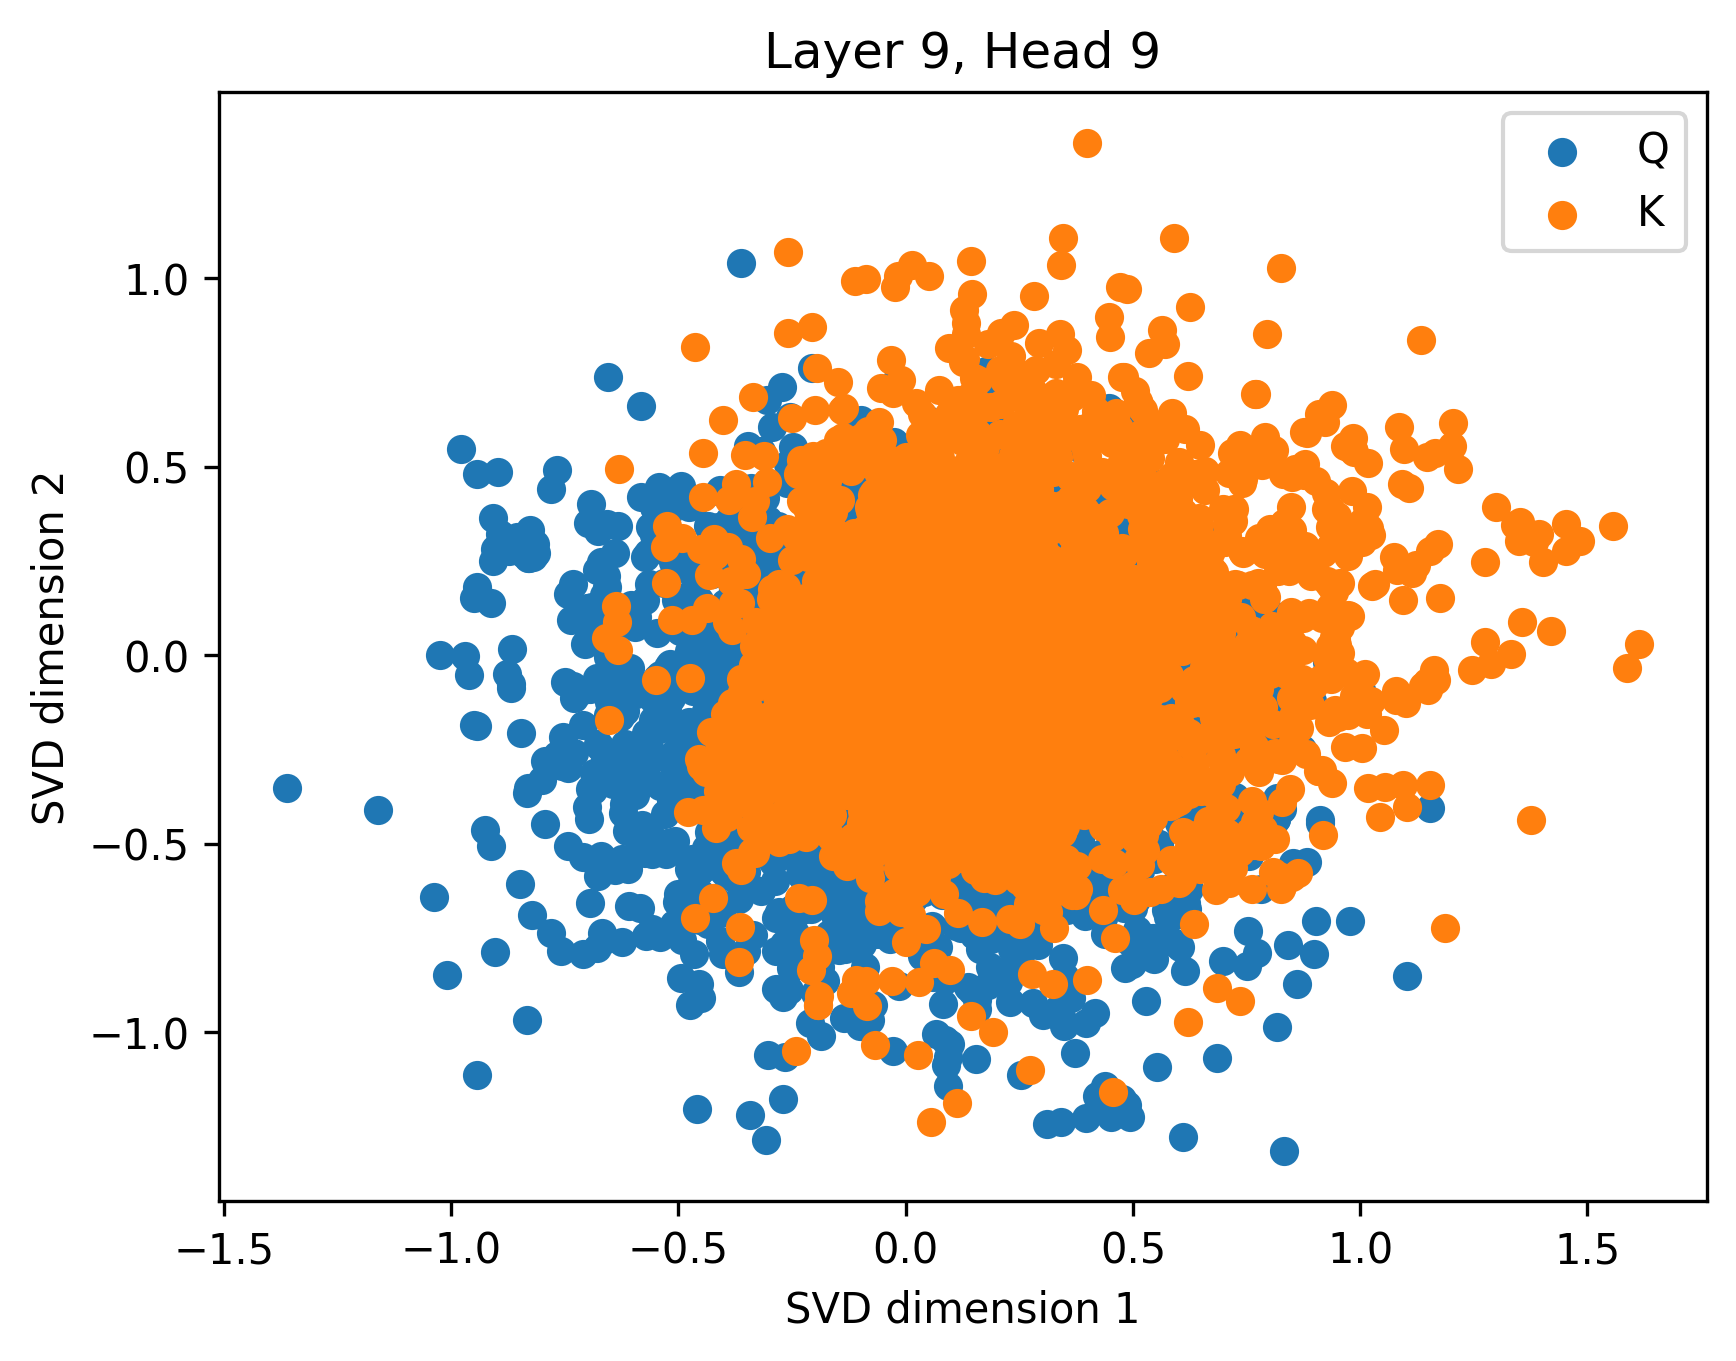
\includegraphics[width=\linewidth]{sources/part_1/anisotropy/imgs/dist_l9h9_s0_K.png}
         \caption{Step 0}
         \label{fig:dist_qk_s0_K}
    \end{subfigure}
    \begin{subfigure}[b]{0.24\linewidth}
         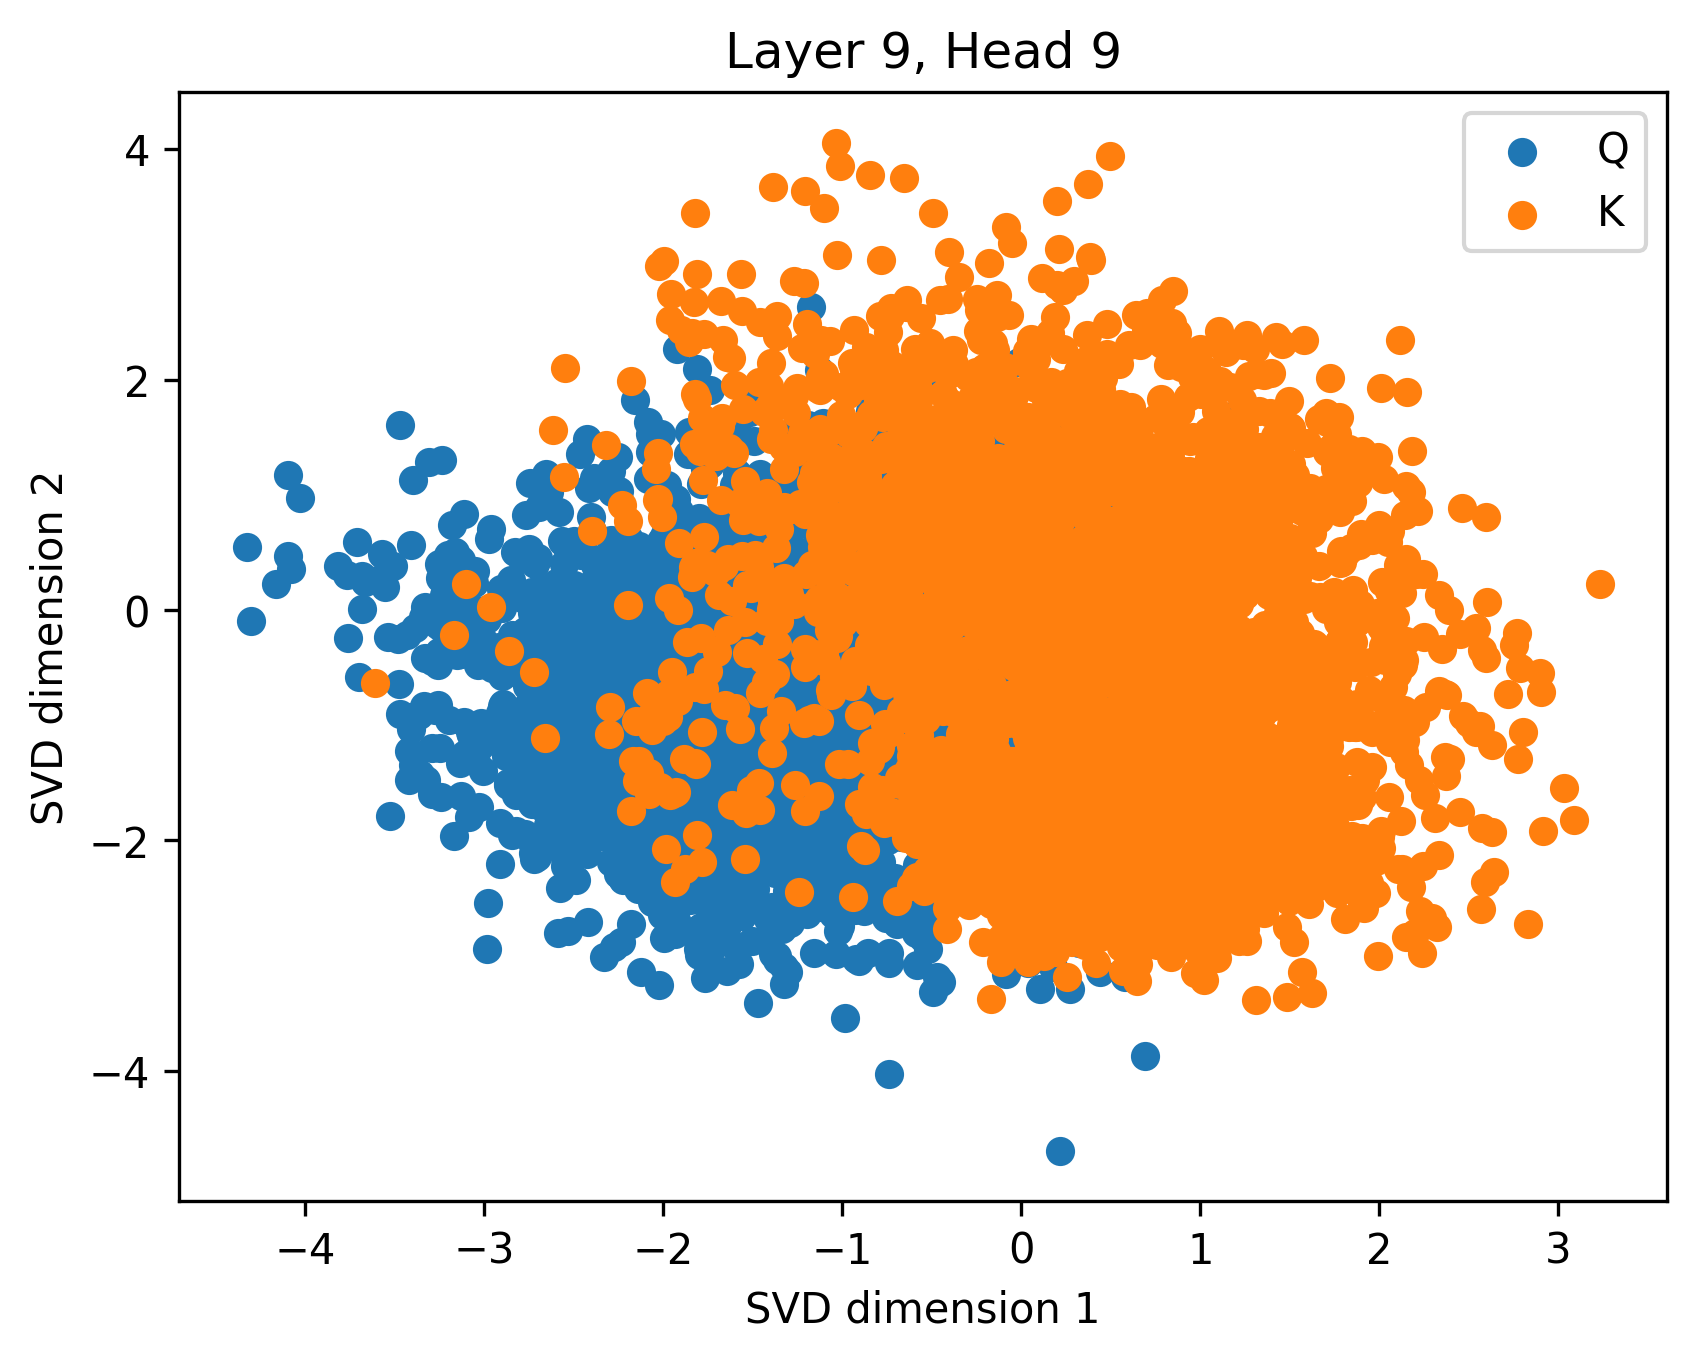
\includegraphics[width=\linewidth]{sources/part_1/anisotropy/imgs/dist_l9h9_s40_K.png}
         \caption{Step 40k}
         \label{fig:dist_qk_s40_K}
    \end{subfigure}
    \begin{subfigure}[b]{0.24\linewidth}
         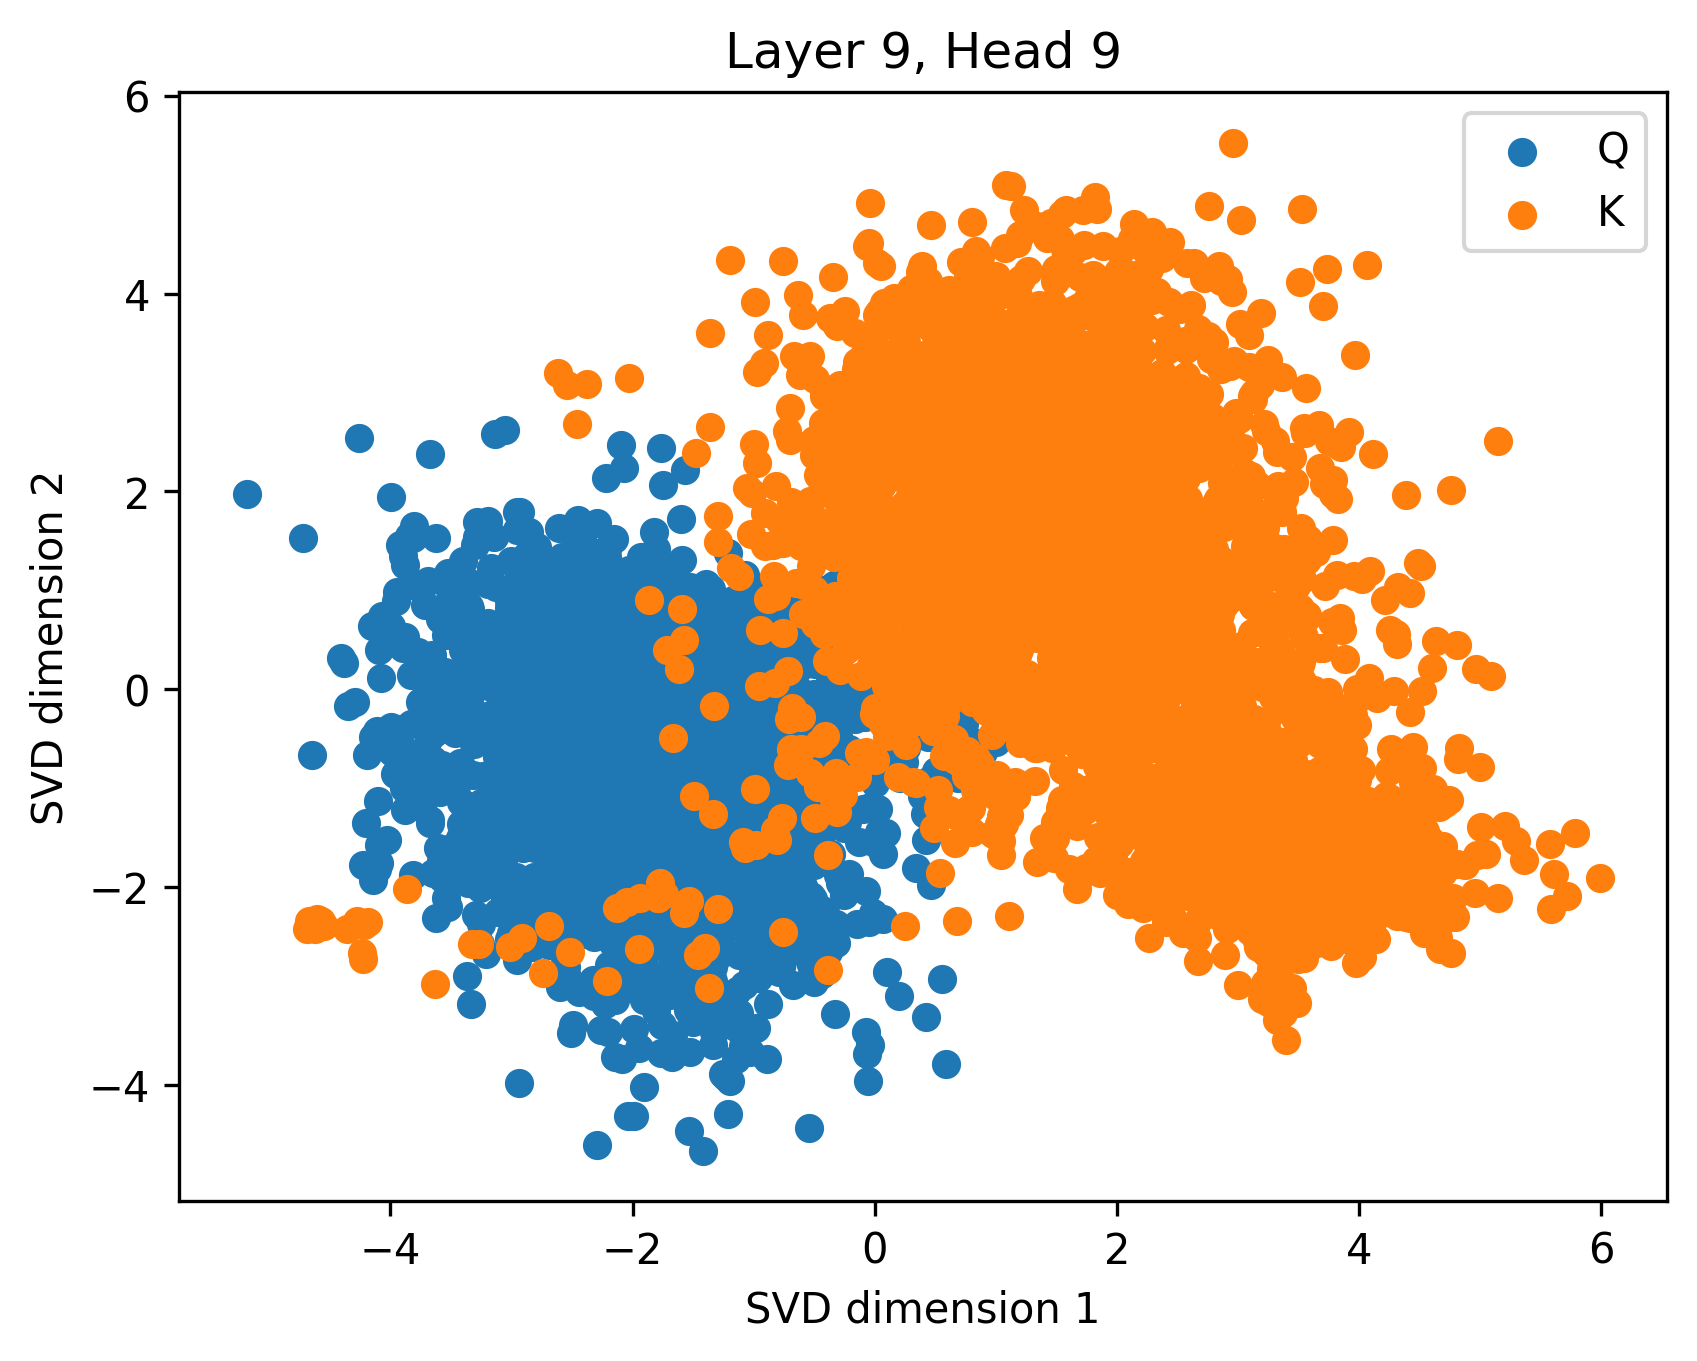
\includegraphics[width=\linewidth]{sources/part_1/anisotropy/imgs/dist_l9h9_s200_K.png}
         \caption{Step 200k}
         \label{fig:dist_qk_s200_K}
    \end{subfigure}
    \begin{subfigure}[b]{0.24\linewidth}
         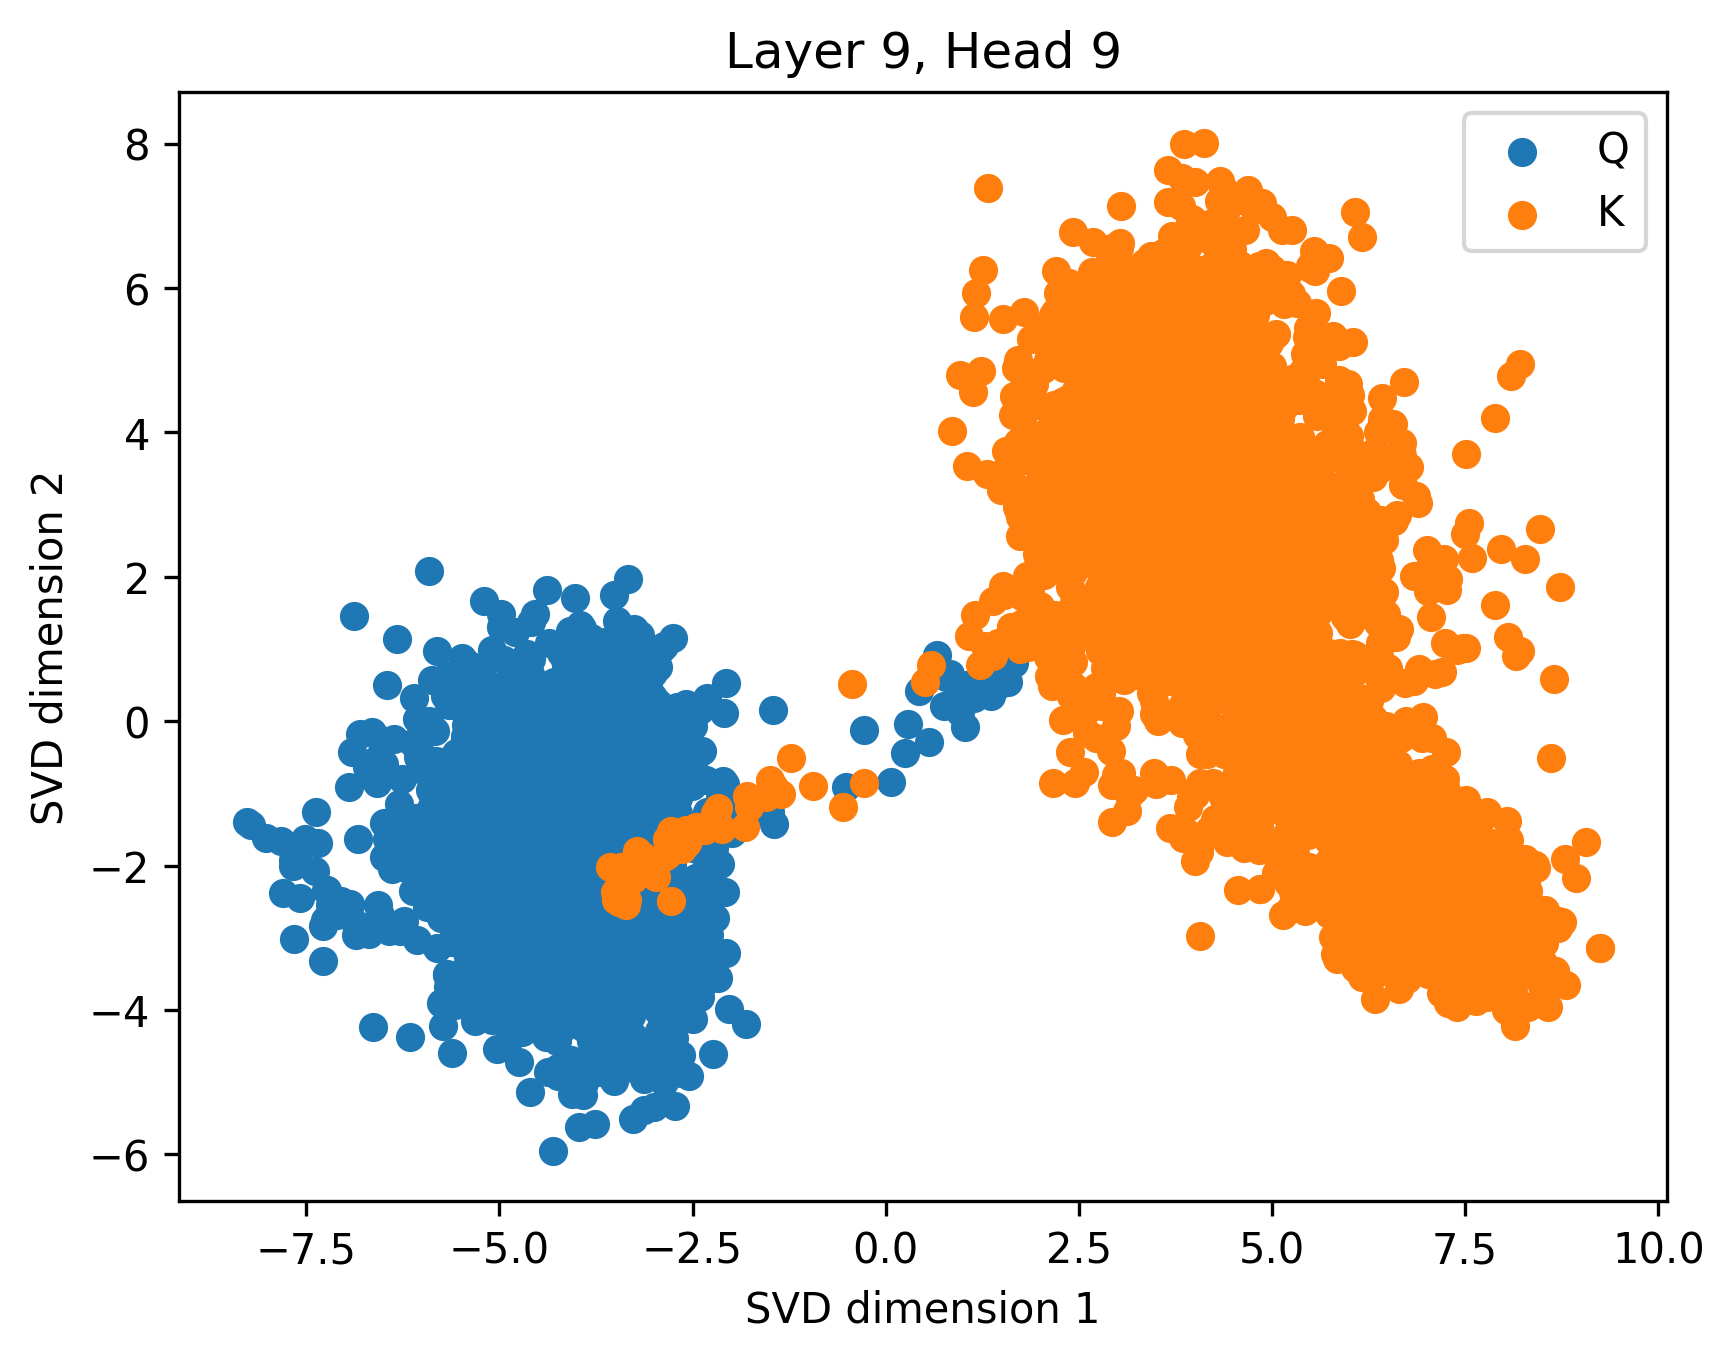
\includegraphics[width=\linewidth]{sources/part_1/anisotropy/imgs/dist_l9h9_s2000_K.png}
         \caption{Step 2M (final)}
         \label{fig:dist_qk_s2M_K}
    \end{subfigure}
    \caption{Evolution of $Q^h_s$ and $K^h_s$ distributions along training. Vectors are projected using the SVD computed on $K^h_s$.}
    \label{fig:proj_qk_heads_K}
\end{figure*}

\begin{figure*}[ht]
    \centering
    \begin{subfigure}[b]{0.24\linewidth}
         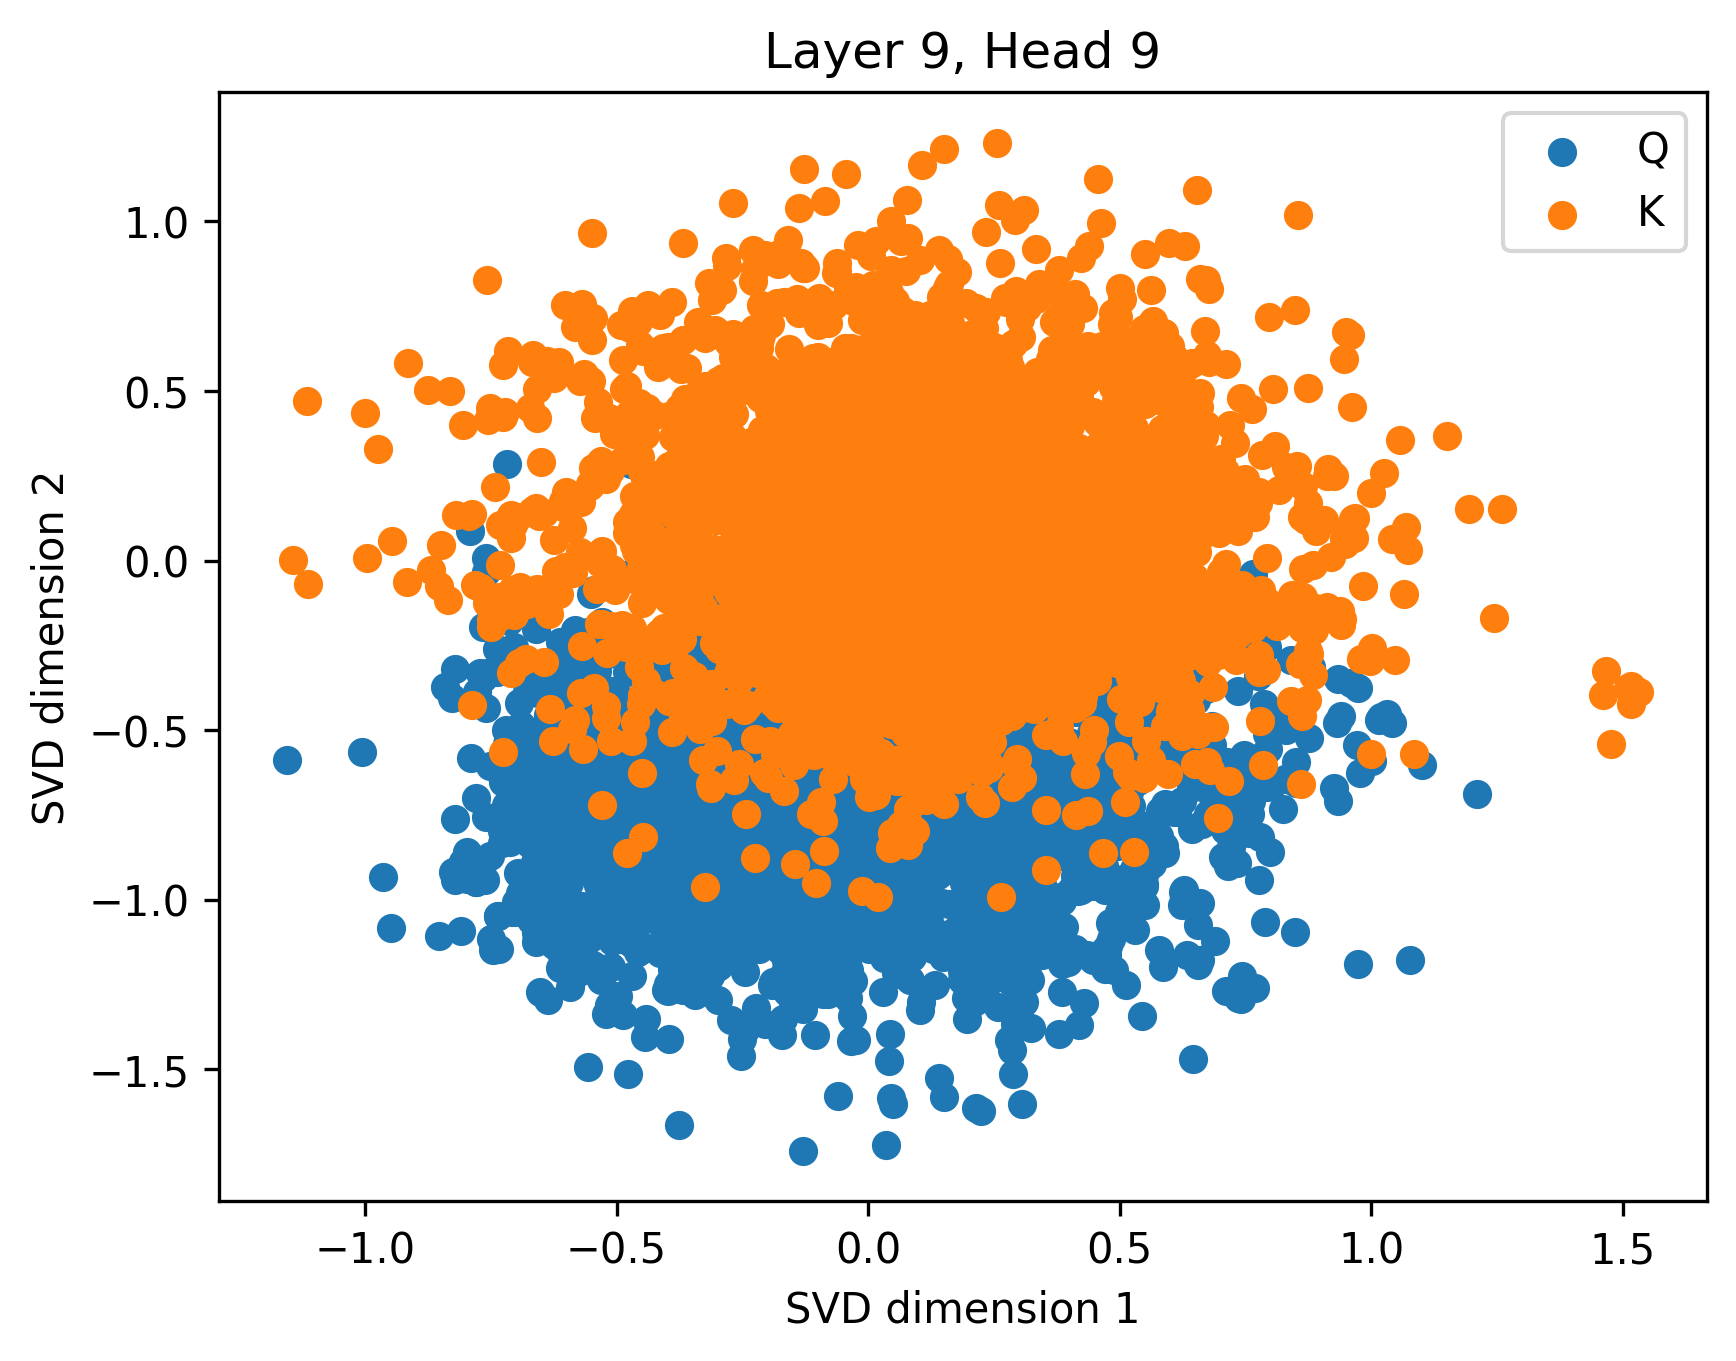
\includegraphics[width=\linewidth]{sources/part_1/anisotropy/imgs/dist_l9h9_s0_Q.png}
         \caption{Step 0}
         \label{fig:dist_qk_s0_Q}
    \end{subfigure}
    \begin{subfigure}[b]{0.24\linewidth}
         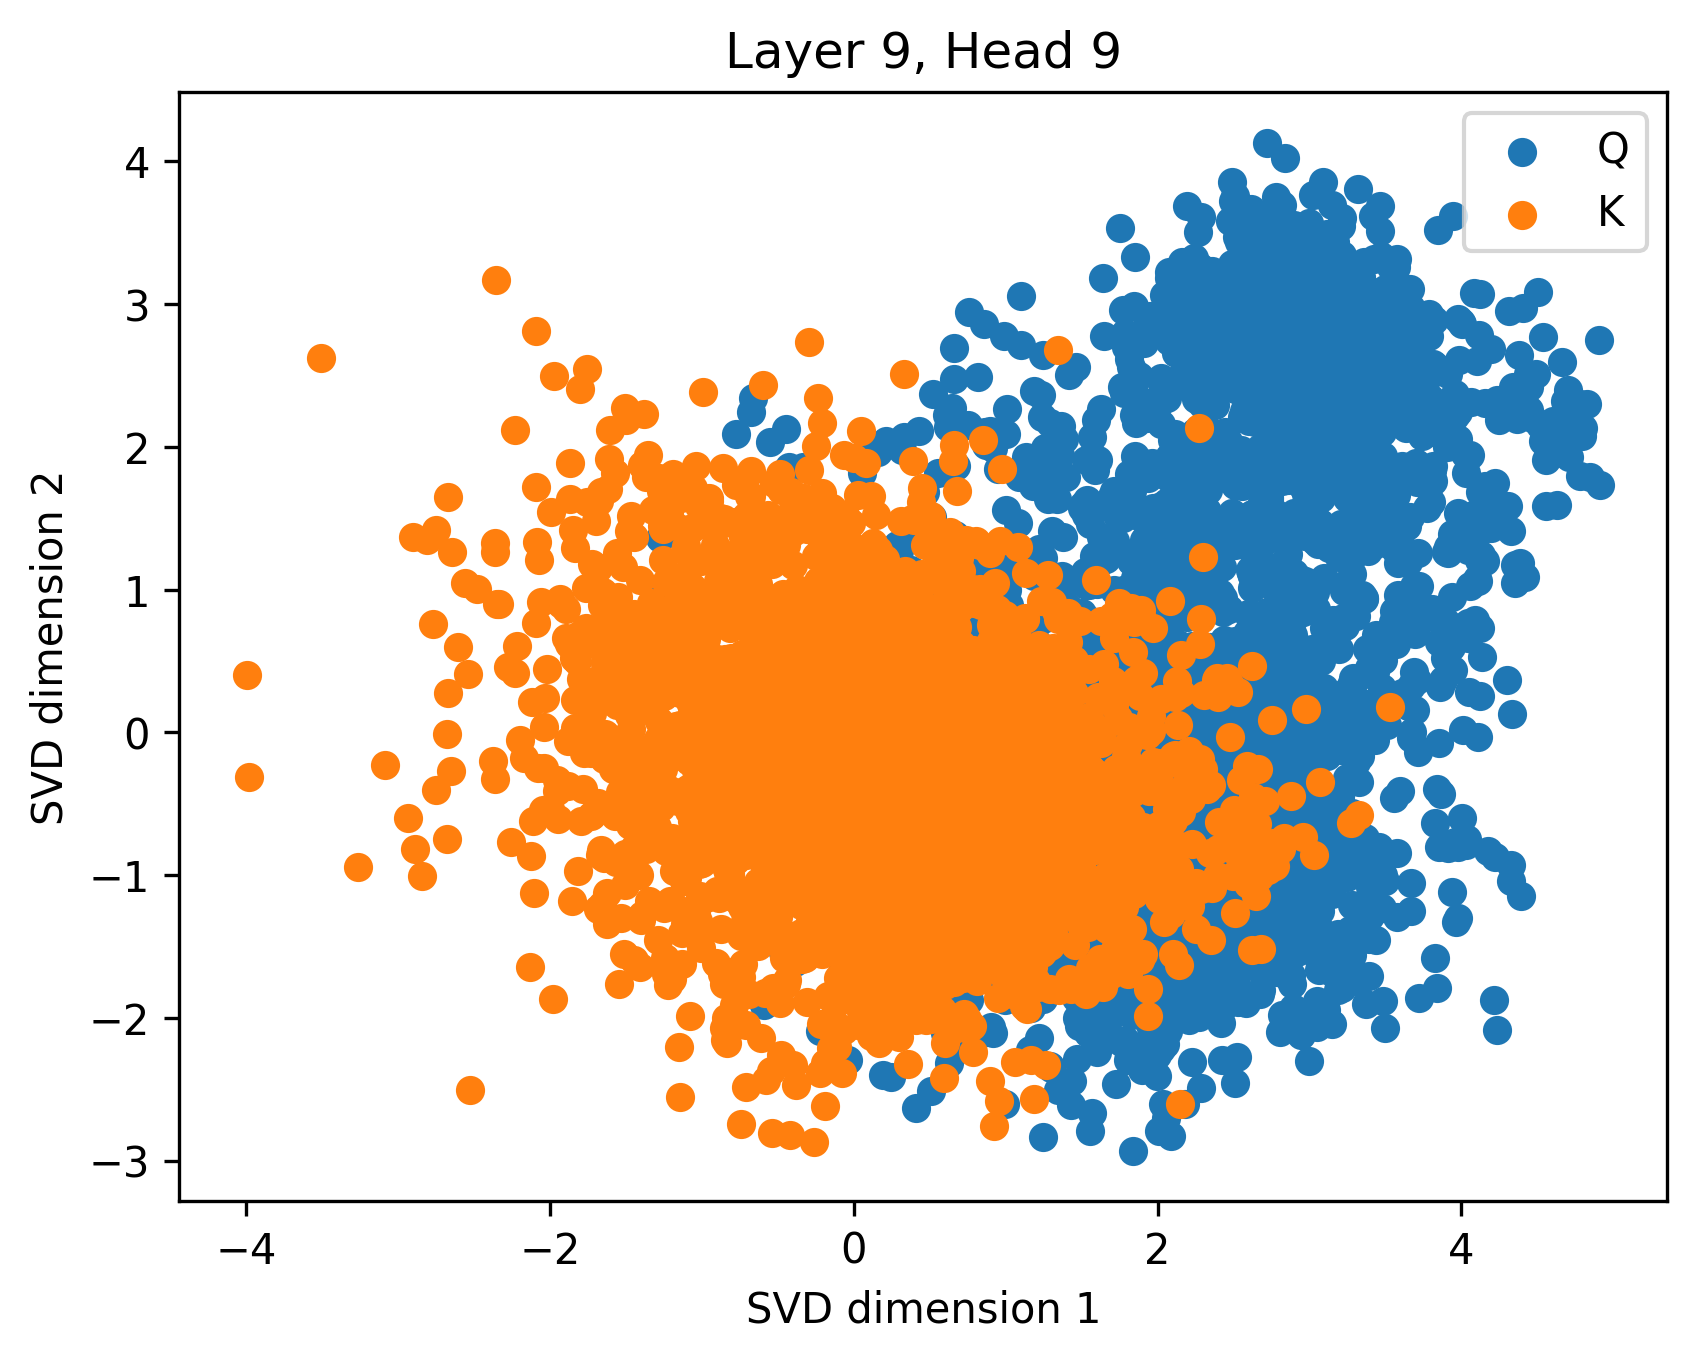
\includegraphics[width=\linewidth]{sources/part_1/anisotropy/imgs/dist_l9h9_s40_Q.png}
         \caption{Step 40k}
         \label{fig:dist_qk_s40_Q}
    \end{subfigure}
    \begin{subfigure}[b]{0.24\linewidth}
         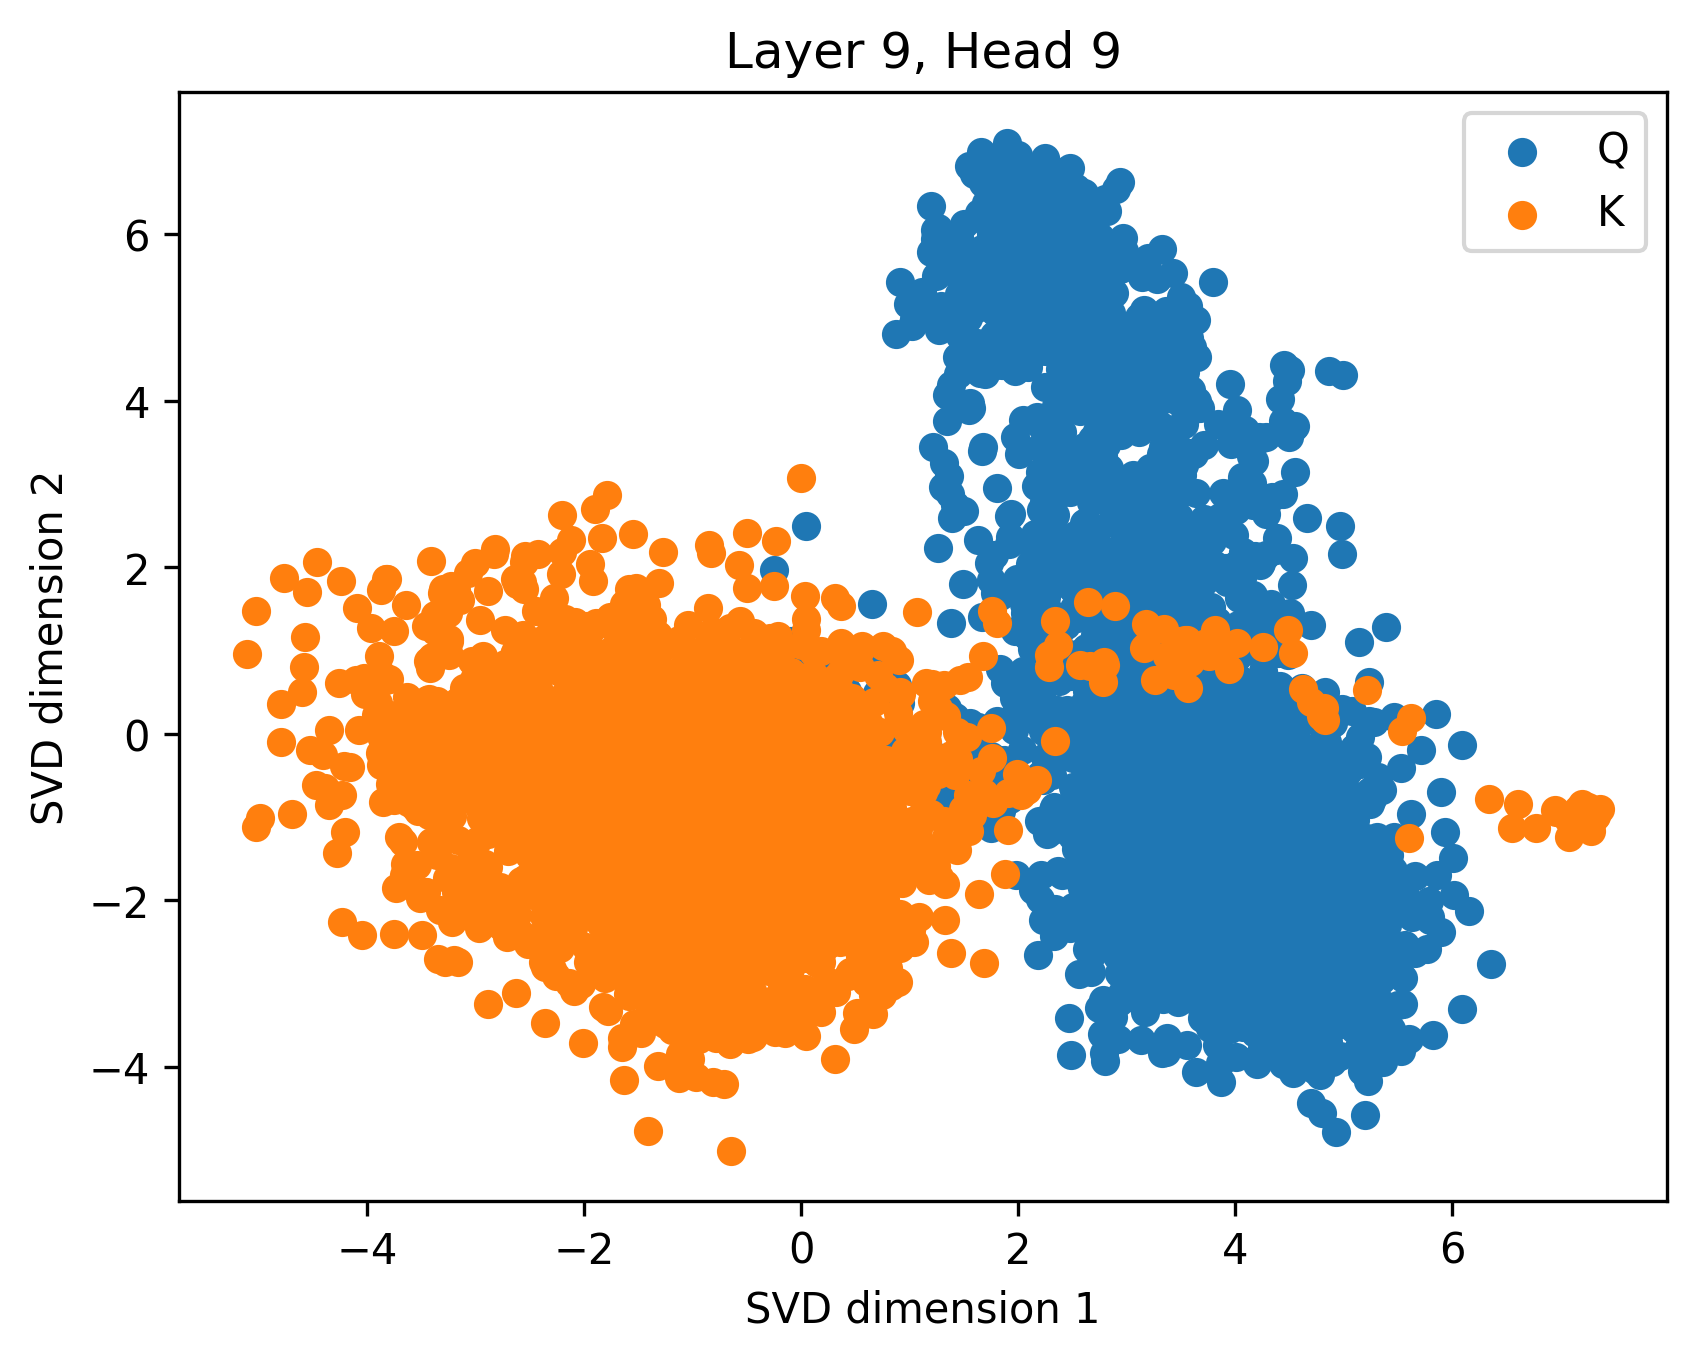
\includegraphics[width=\linewidth]{sources/part_1/anisotropy/imgs/dist_l9h9_s200_Q.png}
         \caption{Step 200k}
         \label{fig:dist_qk_s200_Q}
    \end{subfigure}
    \begin{subfigure}[b]{0.24\linewidth}
         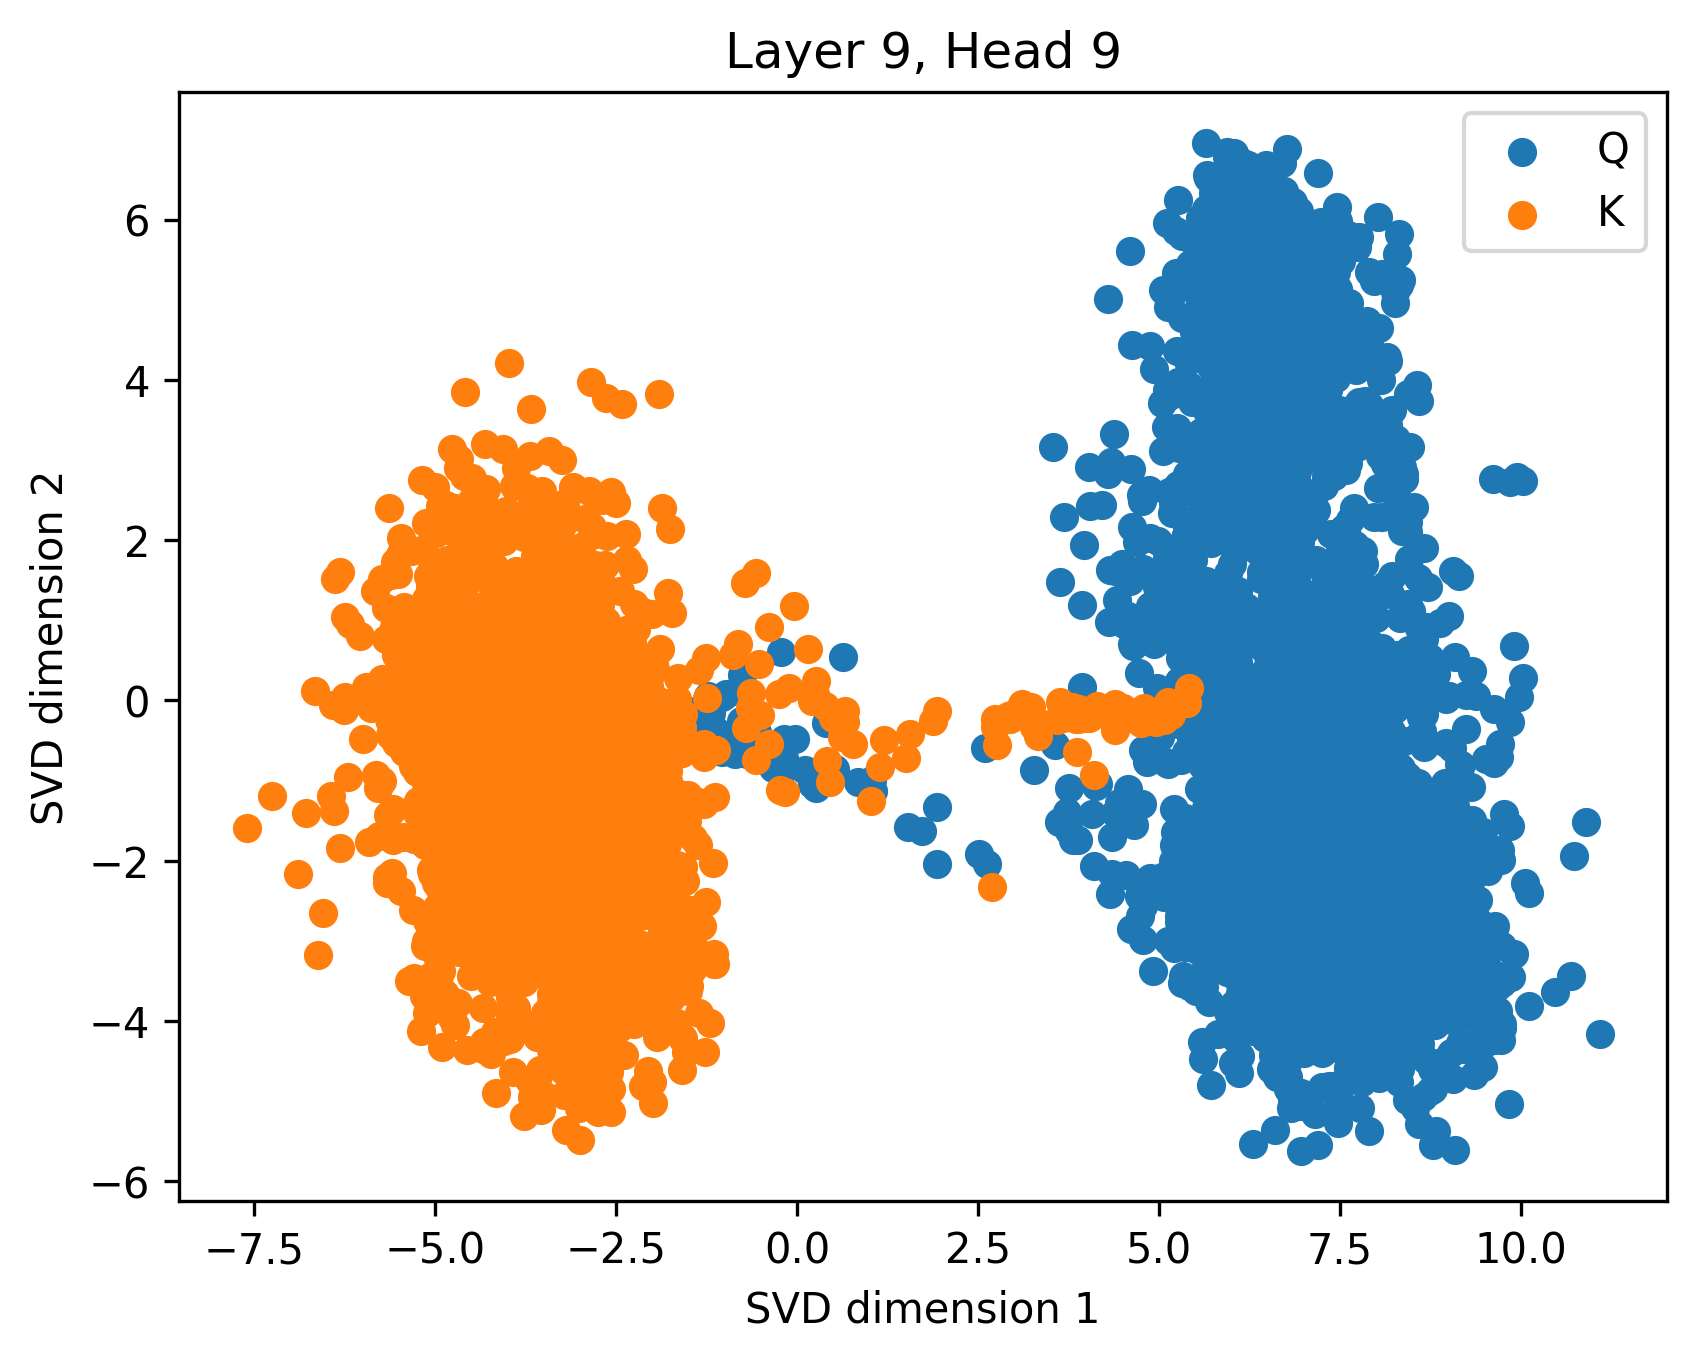
\includegraphics[width=\linewidth]{sources/part_1/anisotropy/imgs/dist_l9h9_s2000_Q.png}
         \caption{Step 2M (final)}
         \label{fig:dist_qk_s2M_Q}
    \end{subfigure}
    \caption{Evolution of $Q^h_s$ and $K^h_s$ distributions along training. Vectors are projected using the SVD computed on $Q^h_s$.}
    \label{fig:proj_qk_heads_Q}
\end{figure*}

\begin{figure}[ht!]
    \centering
    \begin{subfigure}[b]{0.48\columnwidth}
         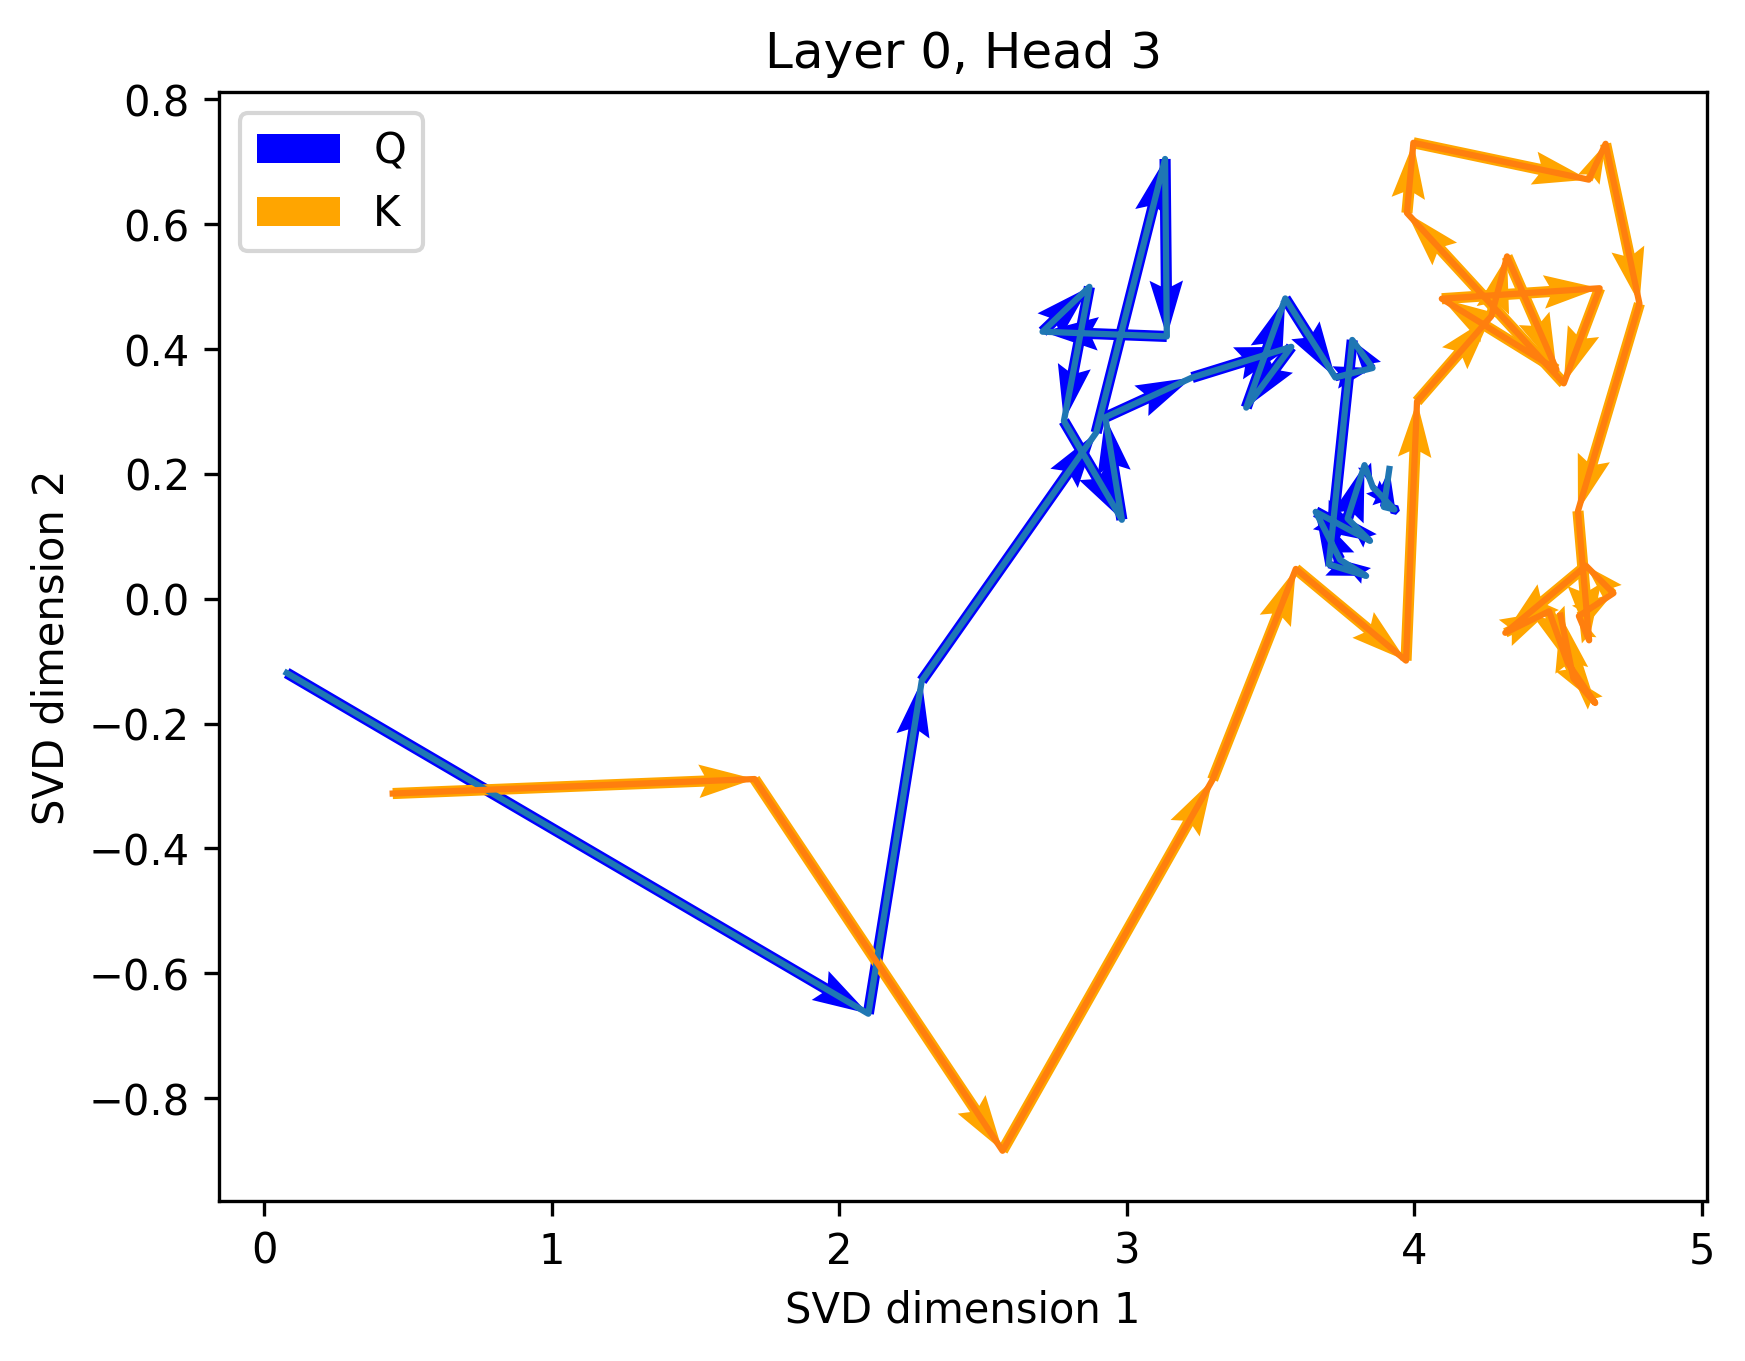
\includegraphics[width=\linewidth]{sources/part_1/anisotropy/imgs/l0h3_samedir_QK_K.png}
         \caption{Similar}
         \label{fig:QK_simdir_K}
    \end{subfigure}
    \begin{subfigure}[b]{0.48\columnwidth}
         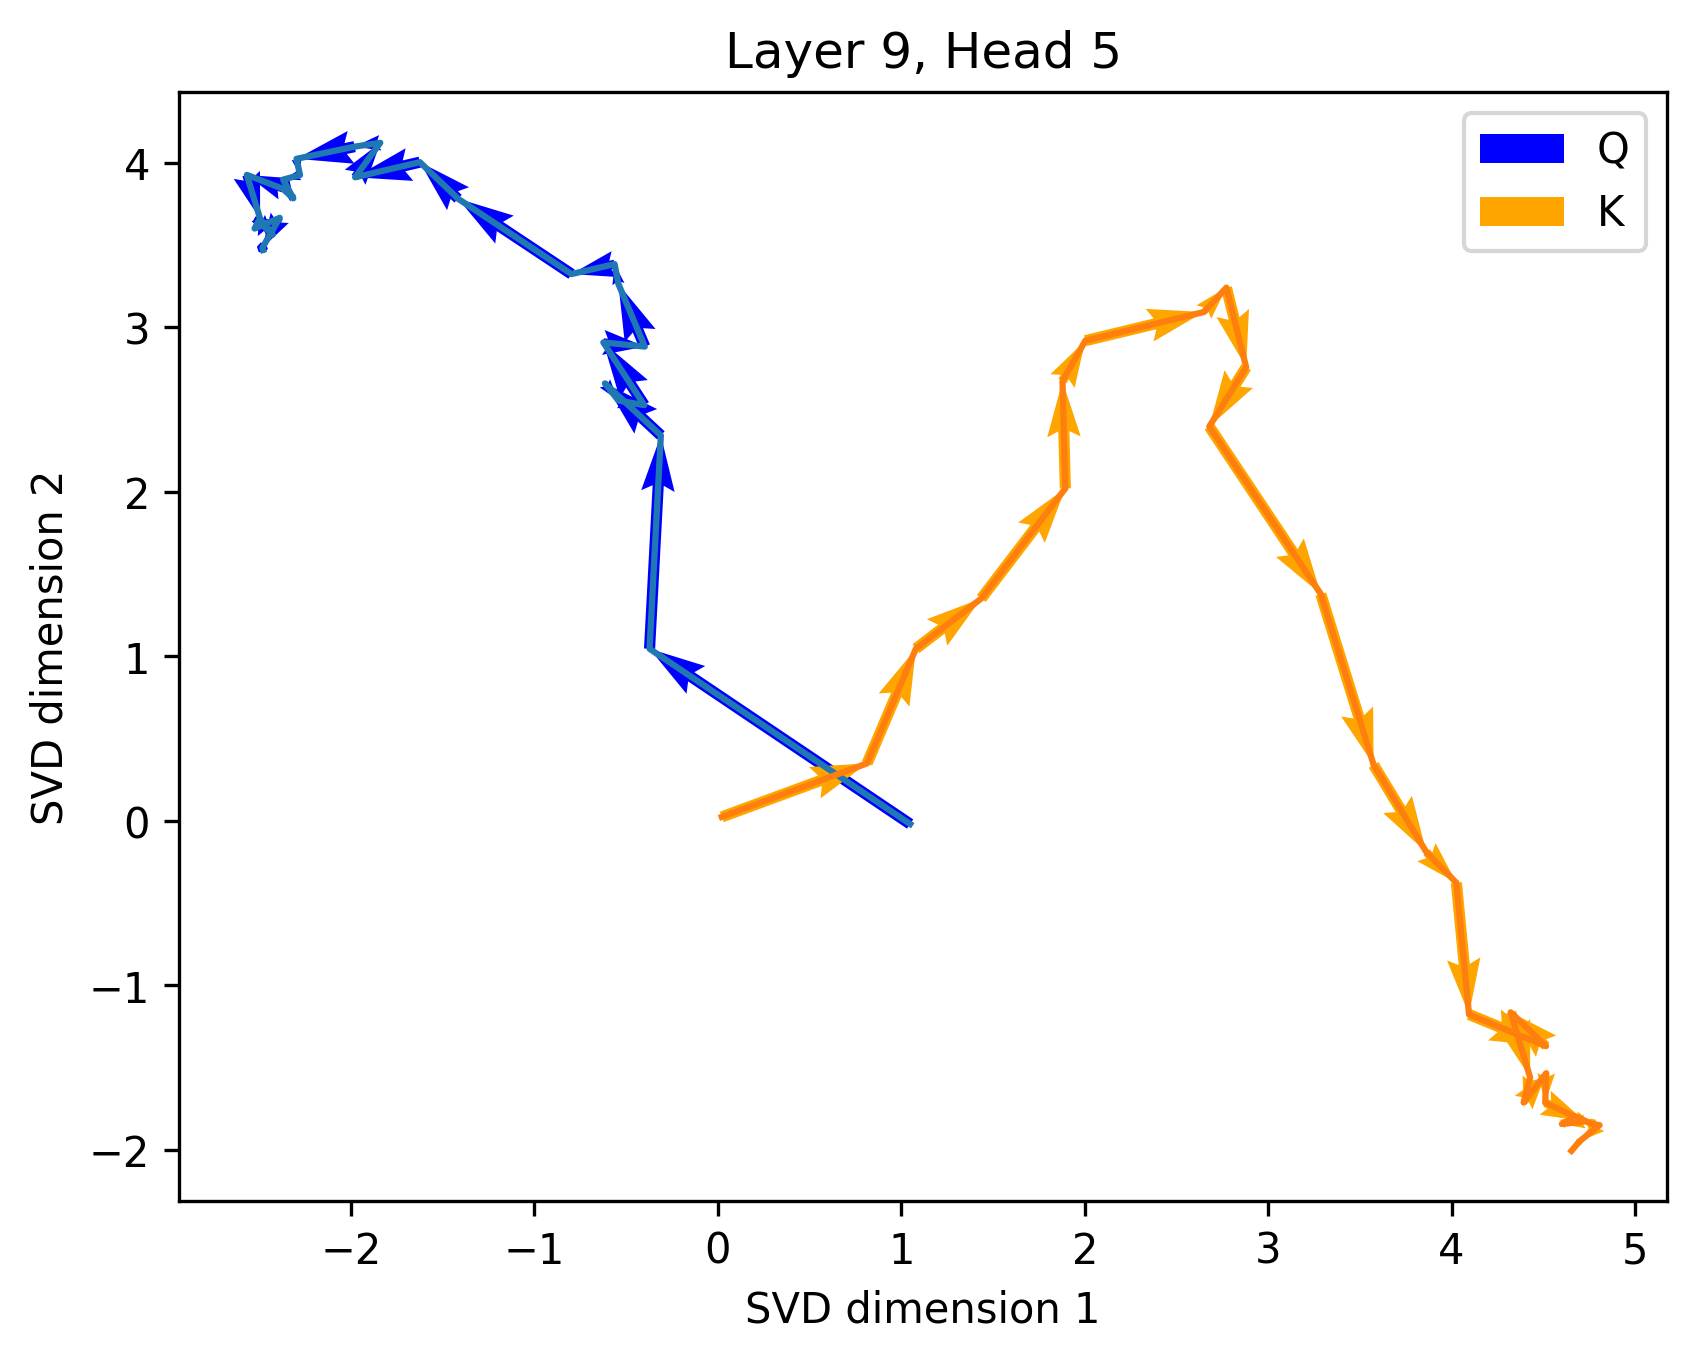
\includegraphics[width=\linewidth]{sources/part_1/anisotropy/imgs/l9h5_diffdir_QK_K.png}
         \caption{Opposite}
         \label{fig:QK_diffdir_K}
    \end{subfigure}
    \caption{Evolution of $\bar{Q^h_s}$ and $\bar{K^h_s}$ along training for two different heads in the network, projected via the SVD of $K^h_s$.
    }
    \label{fig:QK_dir_K}
\end{figure}

\begin{figure}[ht!]
    \centering
    \begin{subfigure}[b]{0.48\columnwidth}
         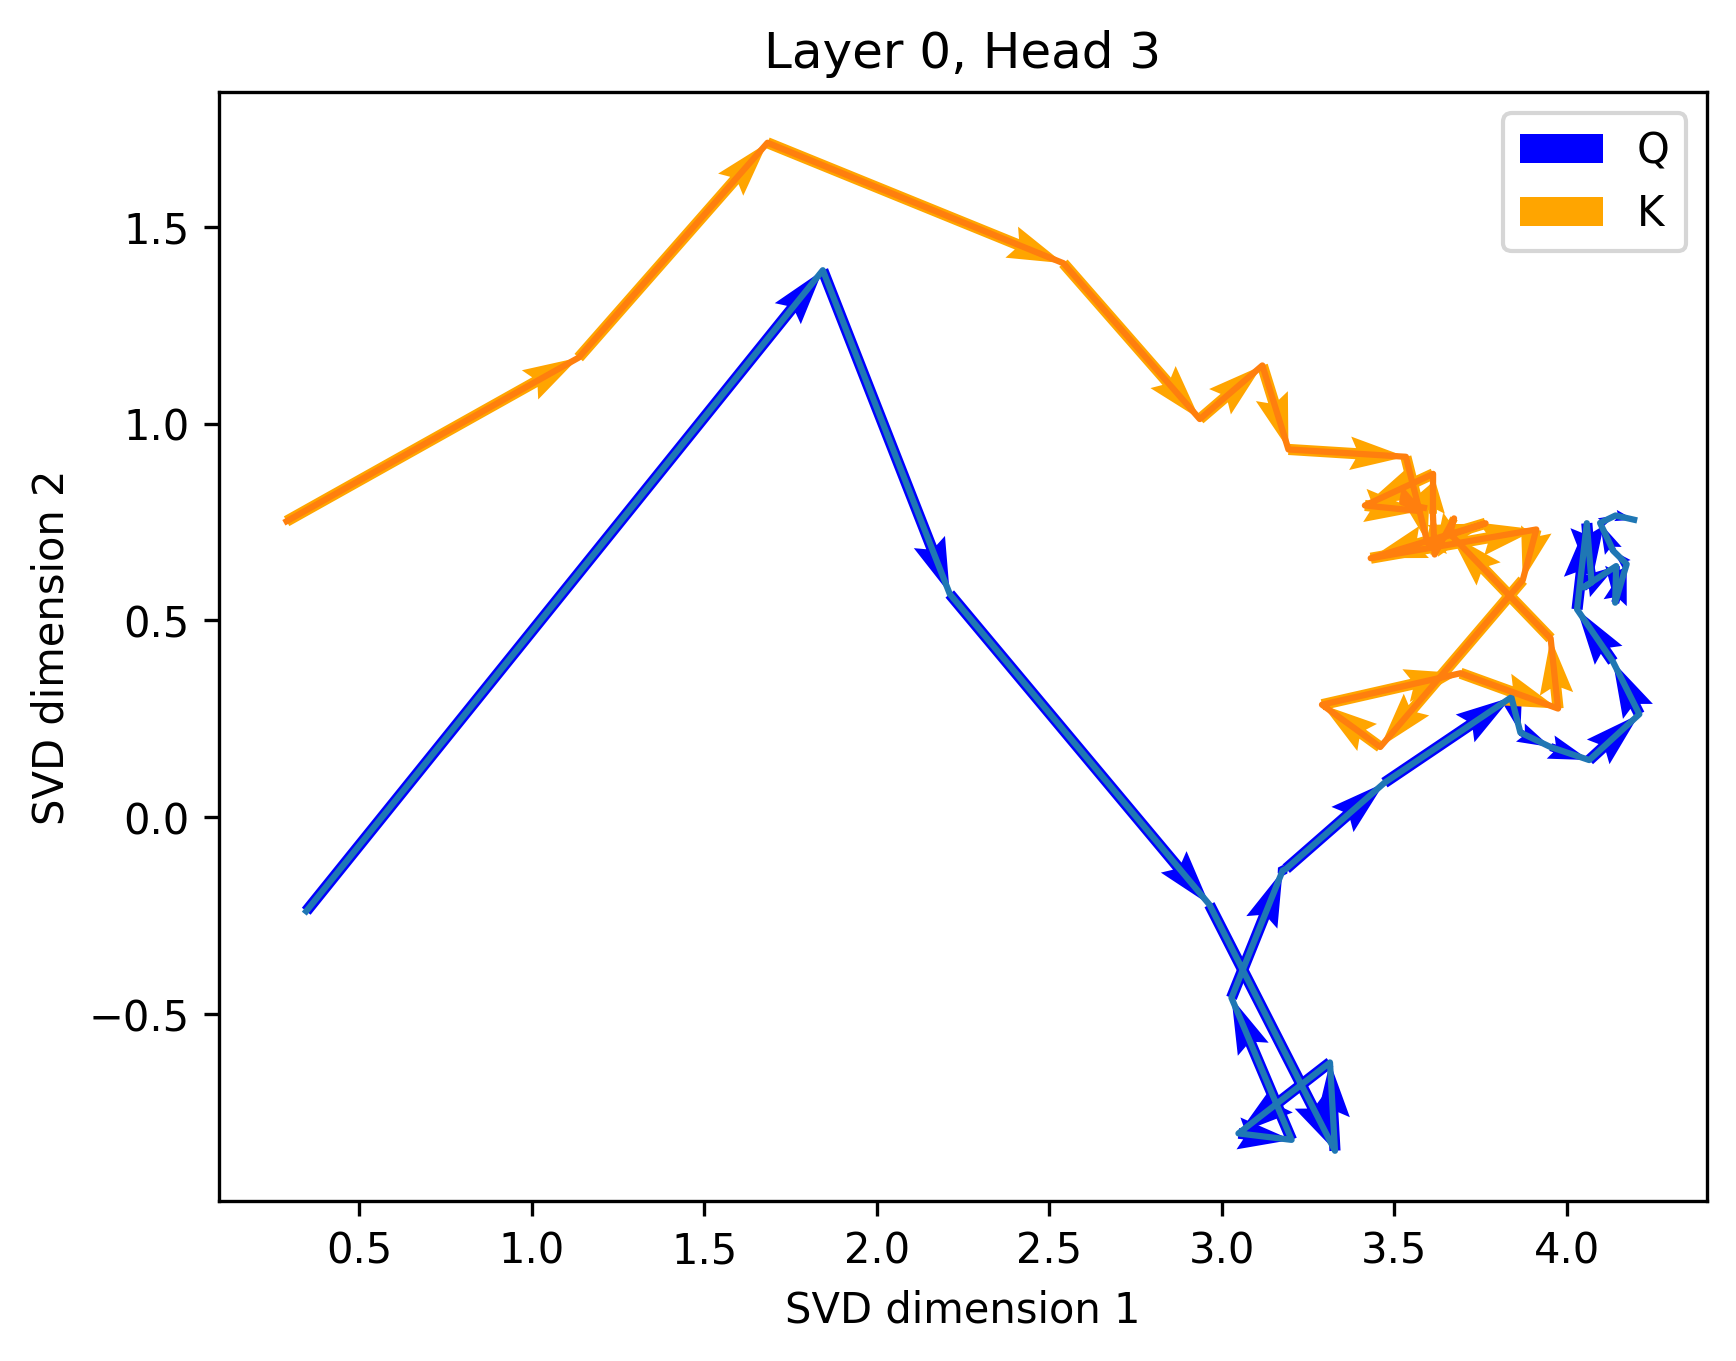
\includegraphics[width=\linewidth]{sources/part_1/anisotropy/imgs/l0h3_samedir_QK_Q.png}
         \caption{Similar}
         \label{fig:QK_simdir_Q}
    \end{subfigure}
    \begin{subfigure}[b]{0.48\columnwidth}
         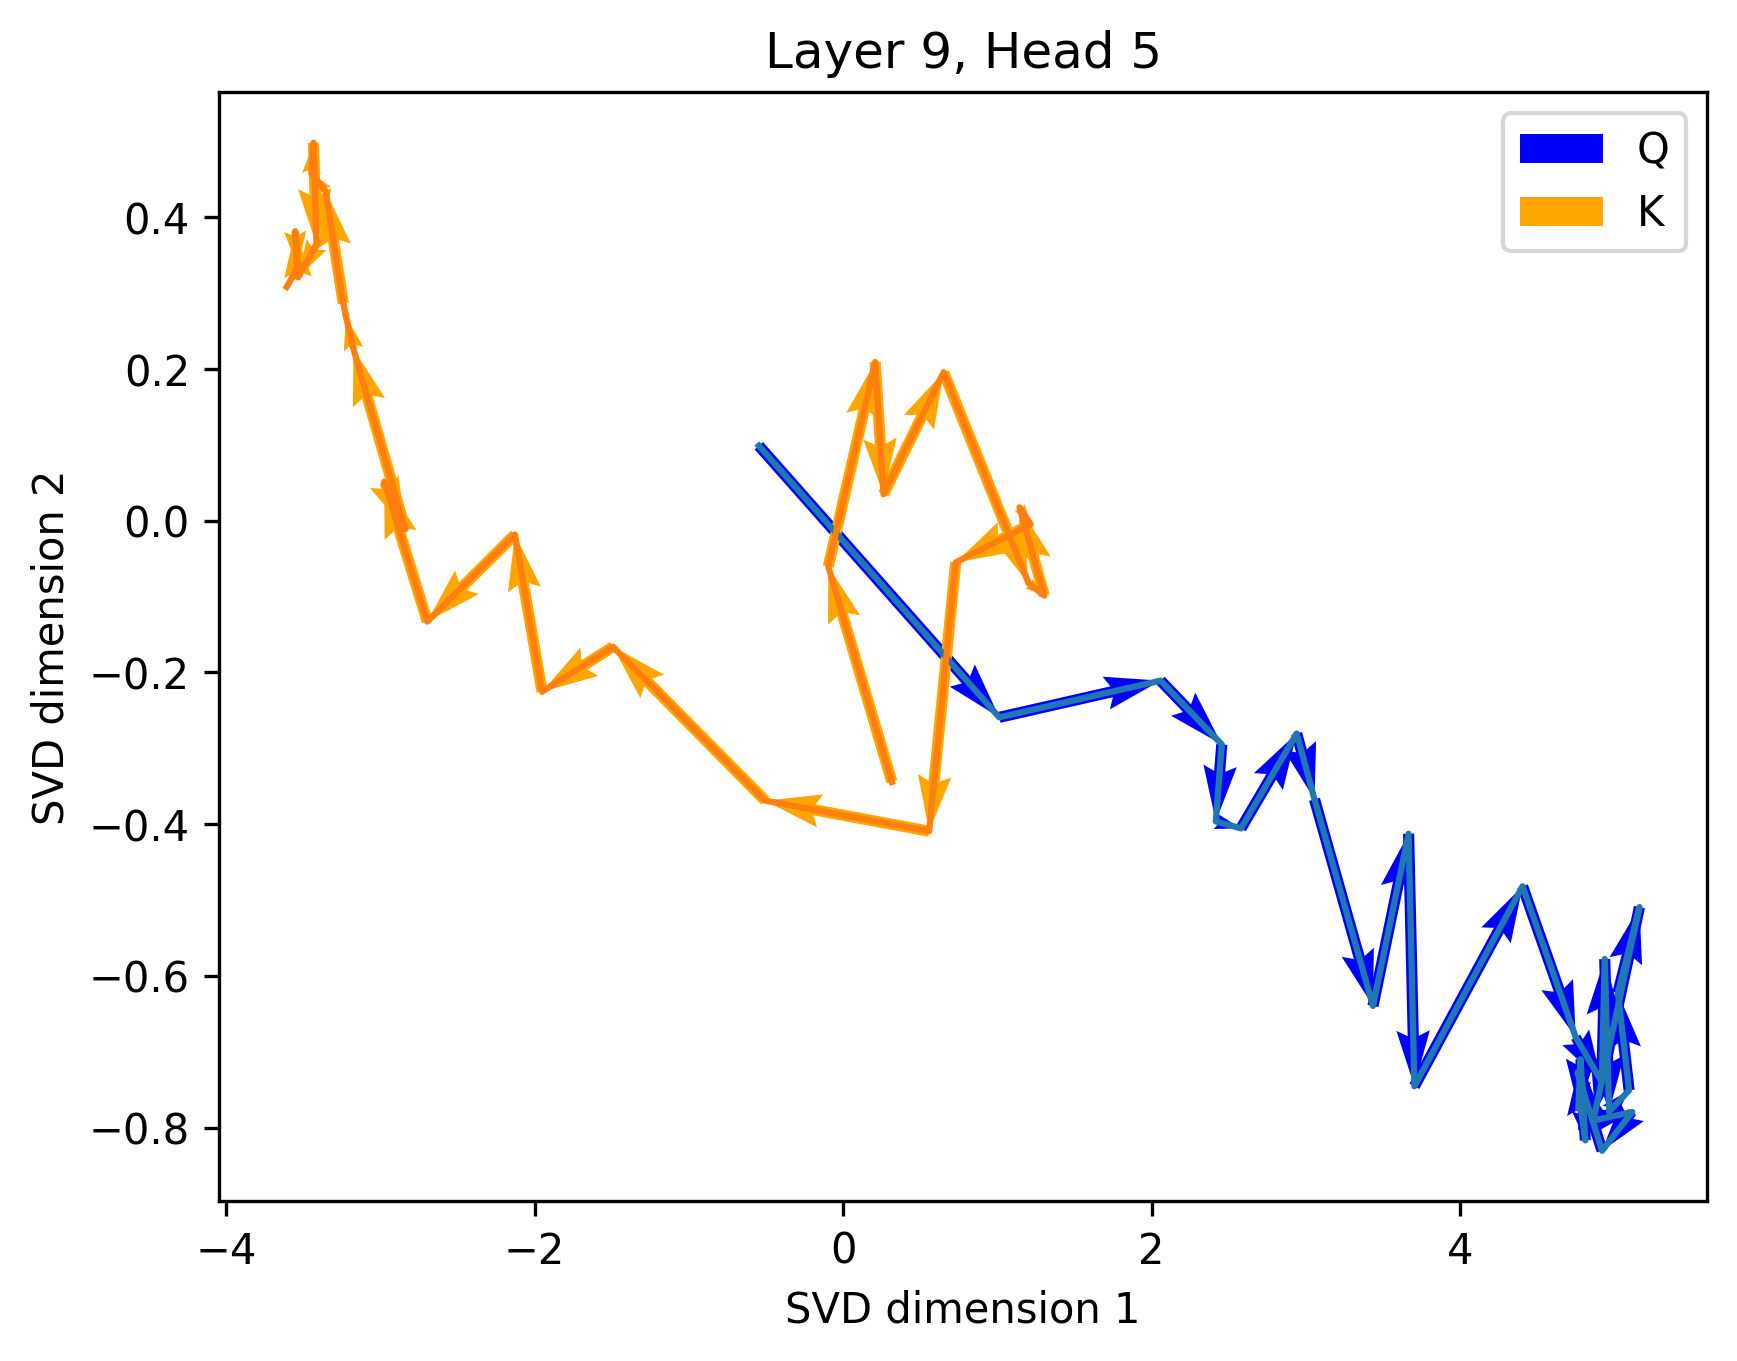
\includegraphics[width=\linewidth]{sources/part_1/anisotropy/imgs/l9h5_diffdir_QK_Q.png}
         \caption{Opposite}
         \label{fig:QK_diffdir_Q}
    \end{subfigure}
    \caption{Evolution of $\bar{Q^h_s}$ and $\bar{K^h_s}$ along training for two different heads in the network, projected via the SVD of $Q^h_s$.}
    \label{fig:QK_dir_Q}
\end{figure}

\subsection{Stability across MultiBERT seeds}
\begin{figure*}[ht]
    \centering
    \begin{subfigure}[b]{0.24\linewidth}
         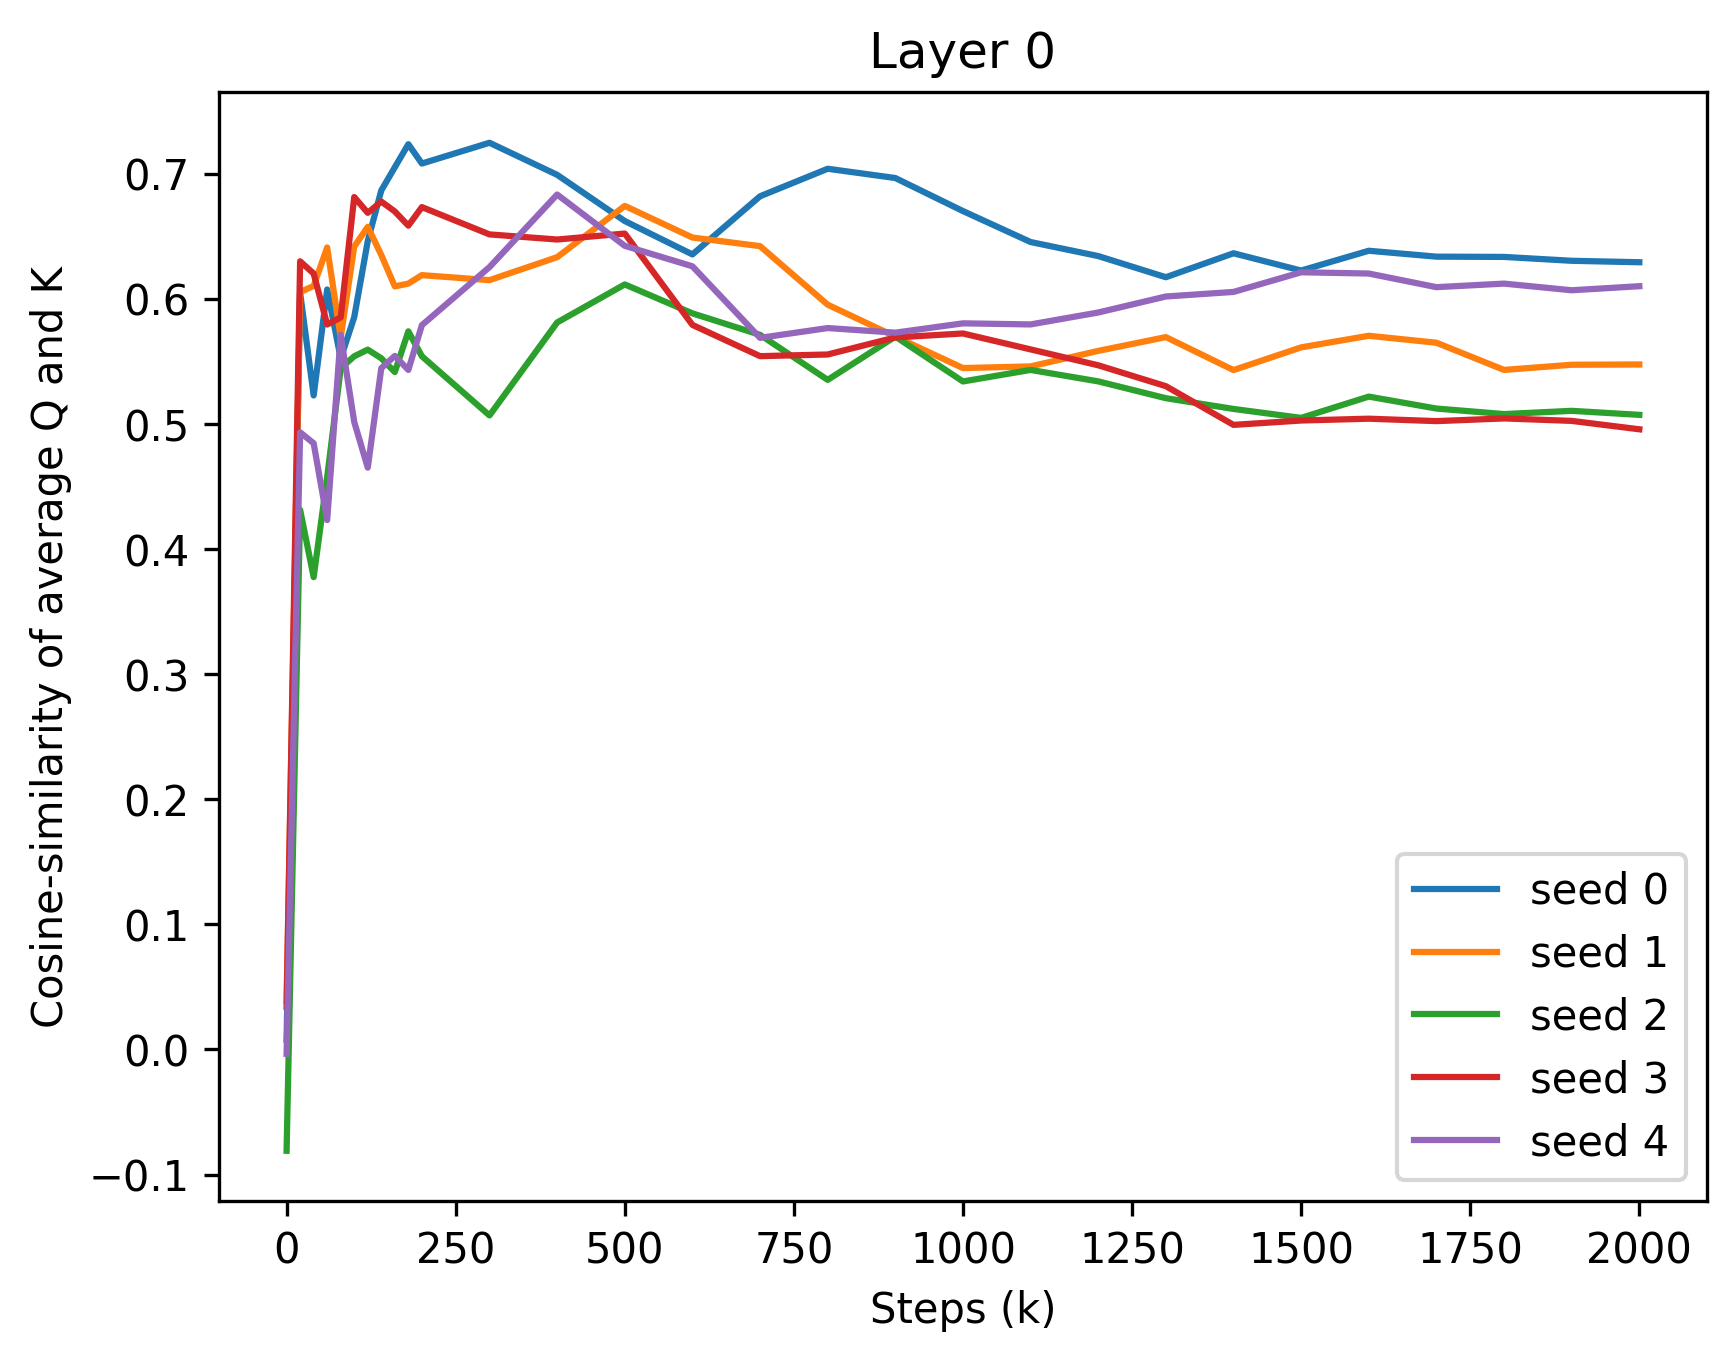
\includegraphics[width=\linewidth]{sources/part_1/anisotropy/imgs/seeds_qk_l0.png}
         \caption{Layer 0}
         \label{fig:seeds_l0}
    \end{subfigure}
    \begin{subfigure}[b]{0.24\linewidth}
         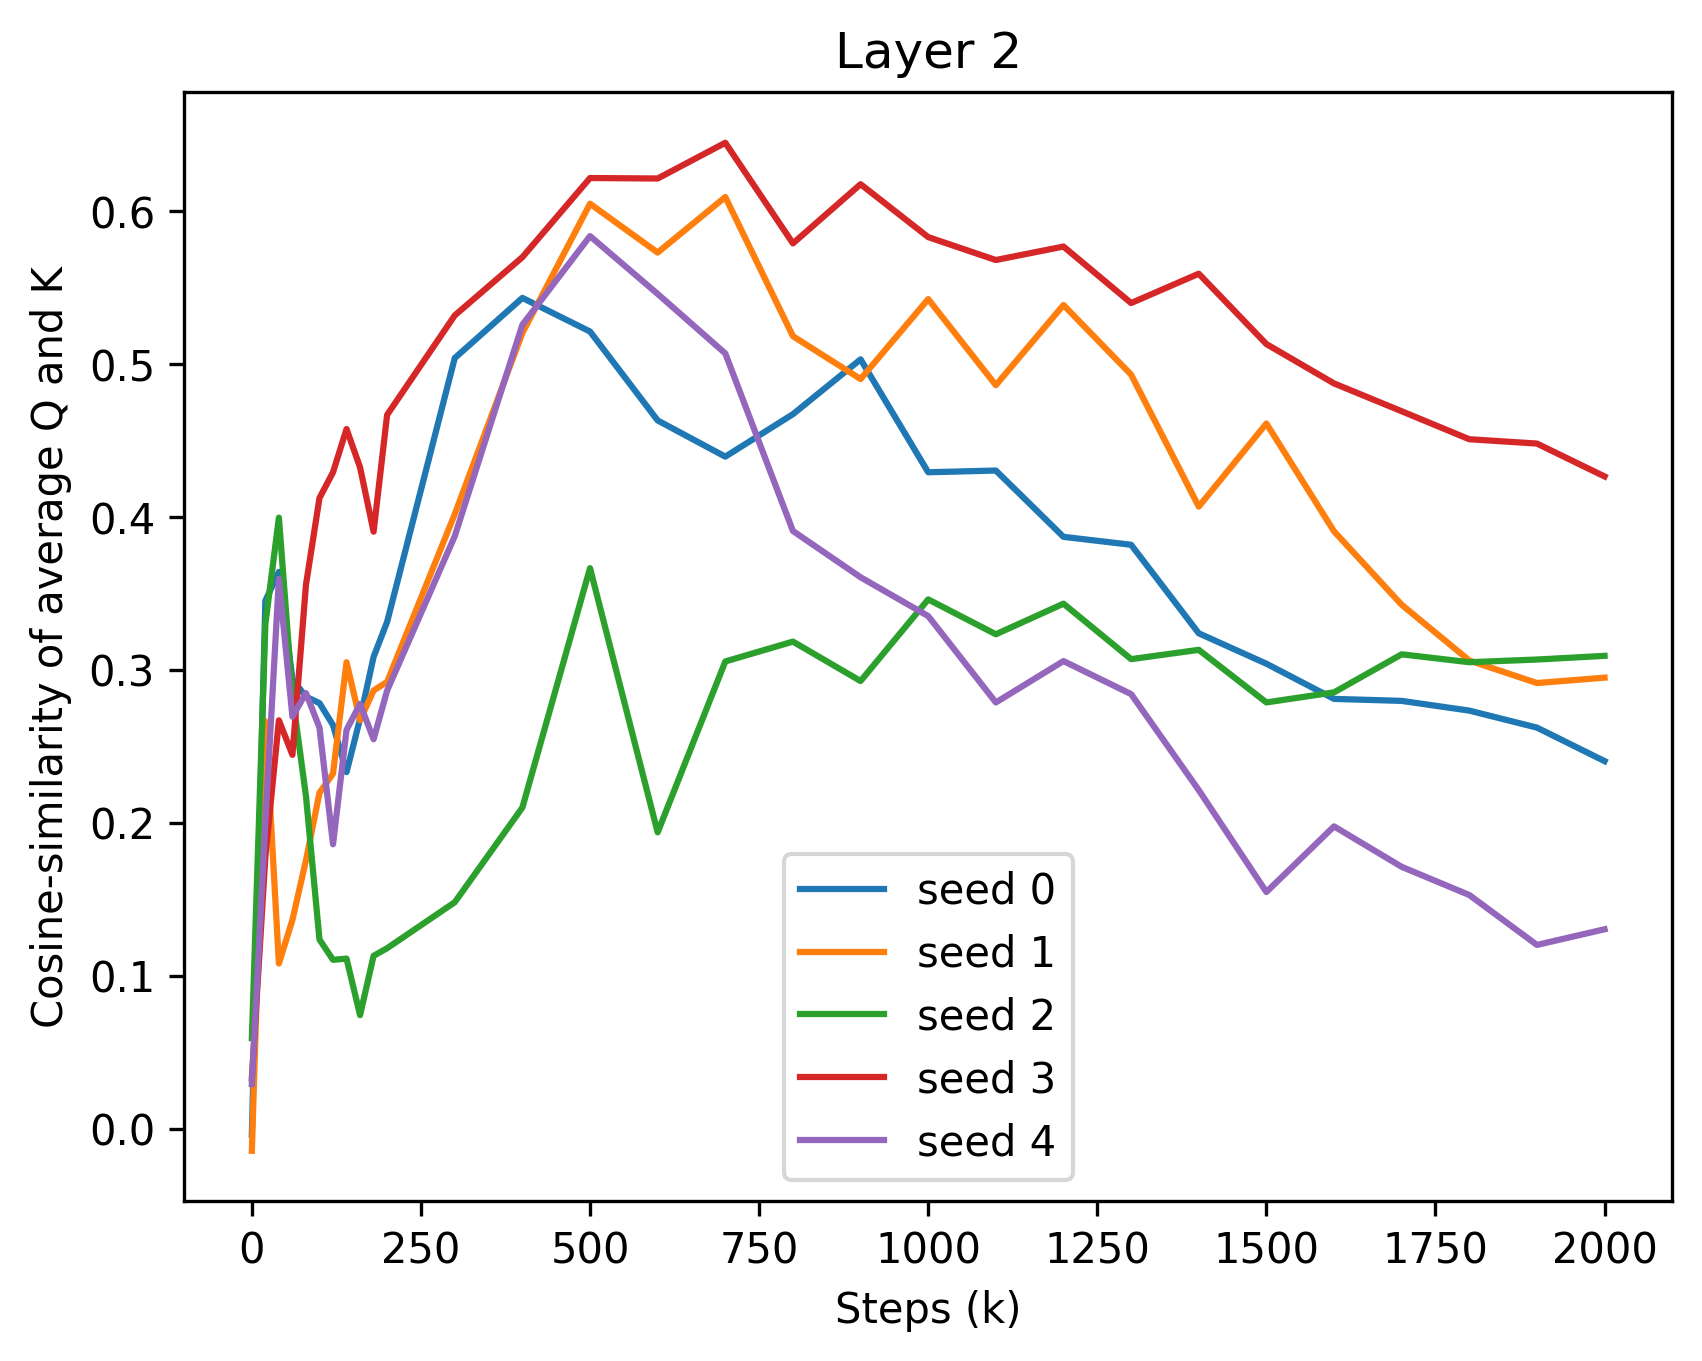
\includegraphics[width=\linewidth]{sources/part_1/anisotropy/imgs/seeds_qk_l2.png}
         \caption{Layer 2}
         \label{fig:seeds_l2}
    \end{subfigure}
    \begin{subfigure}[b]{0.24\linewidth}
         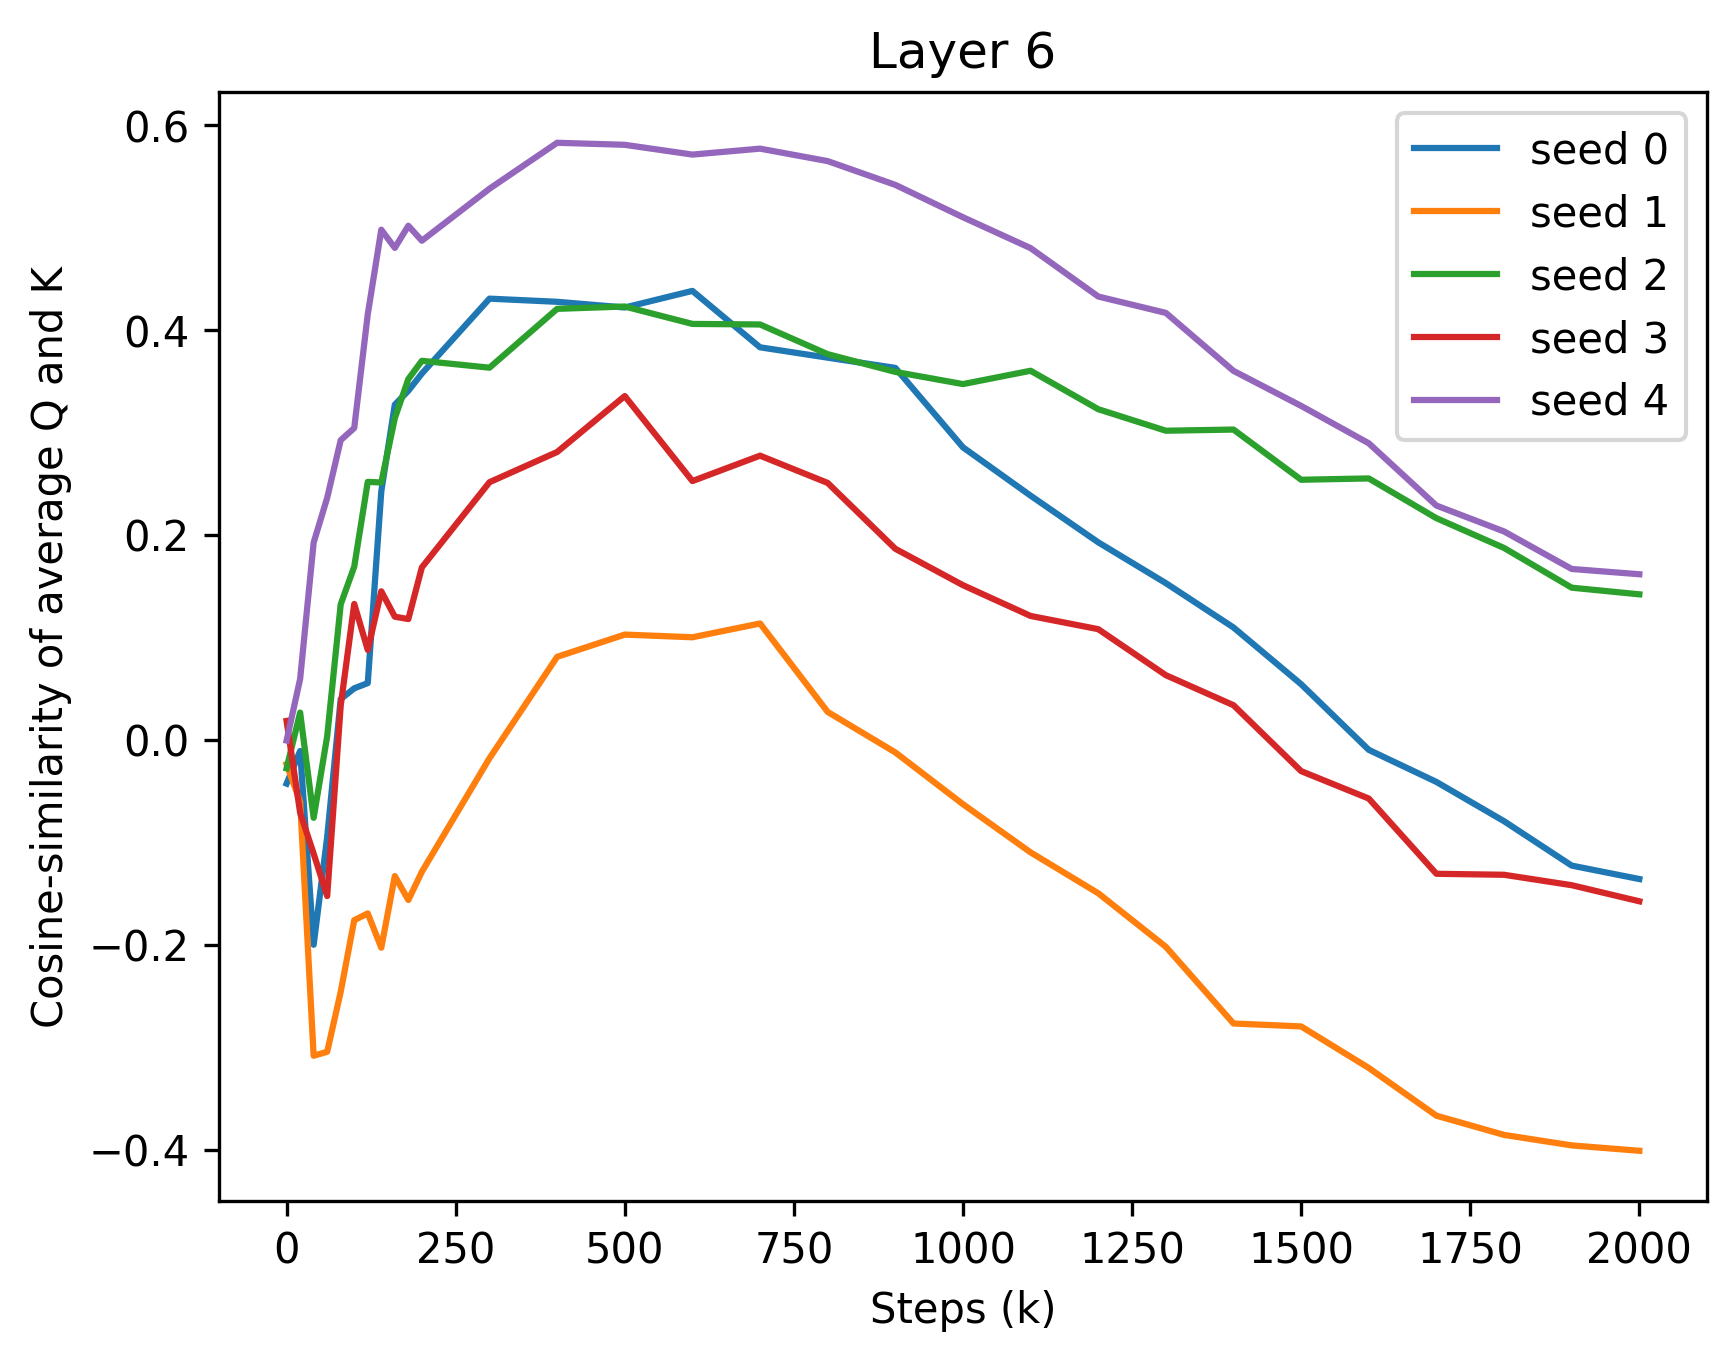
\includegraphics[width=\linewidth]{sources/part_1/anisotropy/imgs/seeds_qk_l6.png}
         \caption{Layer 6}
         \label{fig:seeds_l6}
    \end{subfigure}
    \begin{subfigure}[b]{0.24\linewidth}
         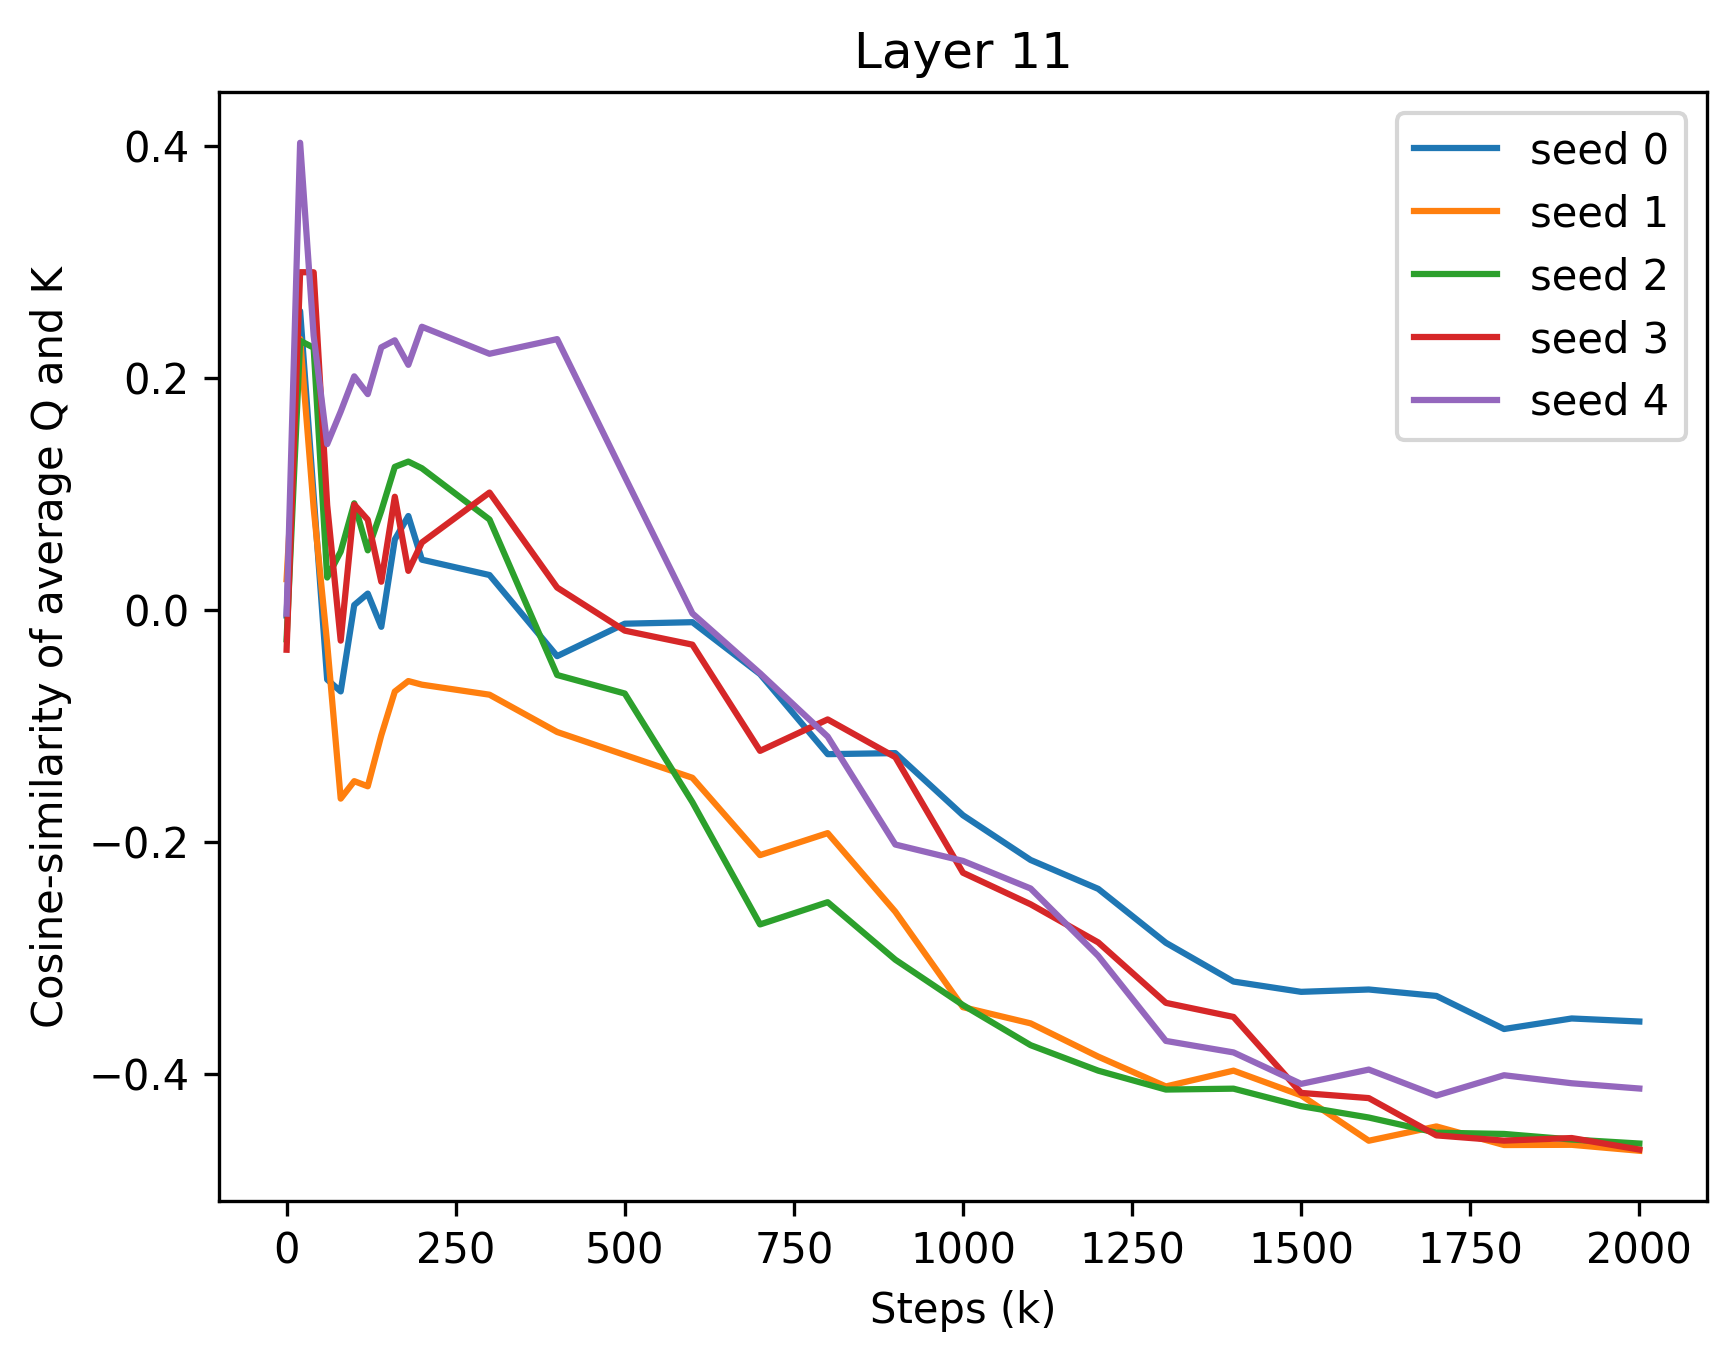
\includegraphics[width=\linewidth]{sources/part_1/anisotropy/imgs/seeds_qk_l11.png}
         \caption{Layer 11}
         \label{fig:seeds_l11}
    \end{subfigure}
    \caption{Evolution of cosine-similarity between $\bar{Q^h_s}$ and $\bar{K^h_s}$ along training for various initialization seeds. Representations are concatenated across heads, and each color represents one seed of the MultiBERT models. We observe similar trends across seeds.}
    \label{fig:seeds_qk}
\end{figure*}

\end{appendices}
